\documentclass[a4paper,openany,12pt]{book}
%\usepackage[utf8]{inputenc}
\usepackage{geometry}
\usepackage[colorlinks,linkcolor=red]{hyperref}
\usepackage{graphicx}
\usepackage{empheq}

\usepackage{amsmath}
\usepackage{amssymb}

\usepackage{multirow}
\usepackage{multicol}
\usepackage{tabularx}

\usepackage{varwidth}
\usepackage{varioref}
\usepackage{cleveref} 
\usepackage{empheq}

\usepackage{picinpar}

\usepackage{appendix}
\usepackage{titling}
\usepackage{uytex}

\usepackage{pgfplots}
\usepackage{tikzpeople}

\usepackage[normalem]{ulem}  %%Wavy line
\usepackage{fontawesome5}

\usetikzlibrary{arrows.meta}

\newcommand\MATH{\textuyghur{ماتېماتىكا}}

%\geometry{left=1.25cm,right=1.25cm,top=1.25cm,bottom=1.25cm}
\geometry{left=1cm,right=1cm,top=1cm,bottom=1cm}
%\geometry{left=3.18cm,right=3.18cm,top=2.54cm,bottom=2.54cm}
%\geometry{inner=2cm,outer=2cm}


\title{ماتېماتىكىدىن ئاساس}
\author{Abdusalam}
\date{\today}

\hypersetup{%
pdftitle = {ماتىماتىكىدىن ئاساس},
pdfsubject = {ماتىماتىكا},
pdfkeywords = {ماتىماتىكا, ئالگېبرا, گېئومتېرىيە},
pdfauthor = {\textcopyright\ Abdusalam},
pdfcreator = {\LaTeX and xeLaTeX},
pdfproducer = {xelatex},
}
%%%%%%%%%%%%%%%%%%%%%%%%%%%%%%%%%%%

\begin{document}
%\includepdf[pages={1}]{chapter/bookcover.pdf}
\clearpage
% command to provide stretchy vertical space in proportion
\newcommand\nbvspace[1][3]{\vspace*{\stretch{#1}}}
% allow some slack to avoid under/overfull boxes
\newcommand\nbstretchyspace{\spaceskip0.5em plus 0.25em minus 0.25em}
% To iسmprove spacing on titlepages
\newcommand{\nbtitlestretch}{\spaceskip0.6em}
\thispagestyle{empty}
\begin{center}
\bfseries
\nbvspace[5]
{\fontsize{36pt}{1.25em}\alkufi \thetitle}
%\HUGE
%{\nbtitlestretch\huge

\nbvspace[3]
\Large {\alelipbe \theauthor}\\[0.5em]
\nbvspace[1]
\normalsize
بۇ قوللانما ئارقىلىق \\
\nbvspace[0.5]
\footnotesize 
سىز  \MATH   بىلىملىرىنى تىزلا كۆرۈپ چىقالايسىز.
\nbvspace[2]


\includegraphics[width=3.5in]{tiger.eps}
\nbvspace[3]
\normalsize

%\today\\
\large
\textenglish{Powered by \LaTeX}
\nbvspace[1]
\end{center}
%يولۋاس مۇقاۋا
\newpage
%\makeatletter
%\@starttoc{toc}
%\makeatother
%title=\textuyghur{\alkufi مۇندەرىجە}
%{\fontsize{16pt}{1.25em}{\alkufi مۇندەرىجە}}
\begin{tcolorbox}[enhanced,title=\textuyghur{{\fontsize{24pt}{1.25em}{\alkufi مۇندەرىجە}}},colframe=blue!50!black,colback=yellow!10!white,colbacktitle=green!55!yellow,breakable,fonttitle=\bfseries,coltitle=black,
attach boxed title to top center={yshift=-0.25mm-\tcboxedtitleheight/2,
yshifttext=2mm-\tcboxedtitleheight/2},boxed title style={boxrule=0.5mm,
frame code={ \path[tcb fill frame] ([xshift=-4mm]frame.west)
-- (frame.north west) -- (frame.north east) -- ([xshift=4mm]frame.east)
-- (frame.south east) -- (frame.south west) -- cycle; },
interior code={ \path[tcb fill interior] ([xshift=-2mm]interior.west)
-- (interior.north west) -- (interior.north east)
-- ([xshift=2mm]interior.east) -- (interior.south east) -- (interior.south west)
-- cycle;} }]
\makeatletter
\@starttoc{toc}
\makeatother
\end{tcolorbox}

%\newpage

%\tableofcontents

\newpage
%%%%%%%%%%%%%%%%%%%%%%%%%%%%%%%%%%%
\setcounter{page}{1}
\part{ئالىي ماتېماتىكا}
\newcommand\yfx{$y=f(x)$}

\mychapter{ئالدىن بىلىملەر}
\par\bigskip
\begin{tcolorbox}
بۇ باپتا ئالىي ماتېماتىكا ئۆگىنىشتىن ئاۋال ھازىرلاشقا تىگىشلىك ئالدىن بىلىملەر خاتېرلەندى. بۇ بىلىملەر ئوتتۇرا مەكتەپ ماتىماتىكا بىلىملىرىدىن ئالىي ماتېماتىكا بىلىملىرىگە بولغان ئۆتكۈنچى نۇقتىلار ھېساپلىنىدۇ.
\end{tcolorbox}

\section{فۇنكىسىيە}
فۇنكسىيەنىڭ ئېنىقلىمىسى ئادەتتە ئەنئەنىۋى ئېنىقلىما ۋە زامانىۋى ئېنىقلىما دەپ ئىككىگە بۆلىنىدۇ. باياننىڭ ئۇقۇمىنىڭ باشلىنىش نۇقتىسى باشقىچە بولغاندىن باشقا ، فۇنكىسىيەنىڭ ئىككى ئېنىقلىمىسى ئاساسەن ئوخشاش. ئەنئەنىۋى ئېنىقلىما ھەرىكەت ئۆزگىرىشى نۇقتىسىدىن باشلىنىدۇ. ، زامانىۋى ئېنىقلىما بولسا توپلام ۋە ئەكىس ئېتىش نۇقتىسىدىن باشلىنىدۇ.

\subsection{ئاساسىي ئېلېمېنتار فۇنكسىيە }
ئاساسىي ئېلېمېنتار فۇنكسىيە تۇراقلىق سان فۇنكسىيەسى، دەرىجە فۇنكسىيەسى، كۆرسەتكۈچلۈك فۇنكسىيە، لوگارىفمىلىق فۇنكسىيە، ترىگونومېتىرىيەلىك فۇنكسىيە، تەتۈر ترىگونومېتىرىيەلىك فۇنكسىيەنى ئۆز ئىچىگە ئالىدۇ. تەپسىلاتى تۆۋەندىكىچە:

تۇراقلىق سان فۇنكسىيەسى
بىرىنچى دەرىجىلىك فۇنكسىيە
ئىككىنچى دەرىجىلىك فۇنكسىيە
تەتۈر تاناسىپلىق فۇنكىسىيە
دەرىجىلىك فۇنكسىيە
كۆرسەتكۈچلۈك فۇنكسىيە
لوگارىفمىلىق فۇنكسىيە
ترىگونومېتىرىيەلىك فۇنكسىيە
تەتۈر ترىگونومېتىرىيەلىك فۇنكسىيە

\subsubsection{تۇراقلىق سان فۇنكسىيەسى}\par\bigskip
%\begin{minipage}{0.35\linewidth}
$y=f(x)=C$ بۇنىڭدا $C$ تۇراقلىق سان. 
%\end{minipage}

\subsubsection{بىرىنچى دەرىجىلىك فۇنكسىيە}
$y=f(x)=ax+b$,$a,b$ خالىغان سان، ھەم
$a \neq 0$

\subsubsection{ئىككىنچى دەرىجىلىك فۇنكسىيە}
$y=f(x)=ax^2+bx+c$,$a,b,c$ خالىغان سان، ھەم
$a \neq 0$

\subsubsection{تەتۈر تاناسىپلىق فۇنكىسىيە}
$y=f(x)=\frac{a}{x}$,$a$ خالىغان سان.

\subsubsection{دەرىجىلىك فۇنكسىيە}\par\bigskip
$y=x^{\mu}$، $\mu$ خالىغان سان\\
$x>0$، $y=x^{\mu}$ رەسىمدىكىدەك بولىدۇ.
\begin{center}
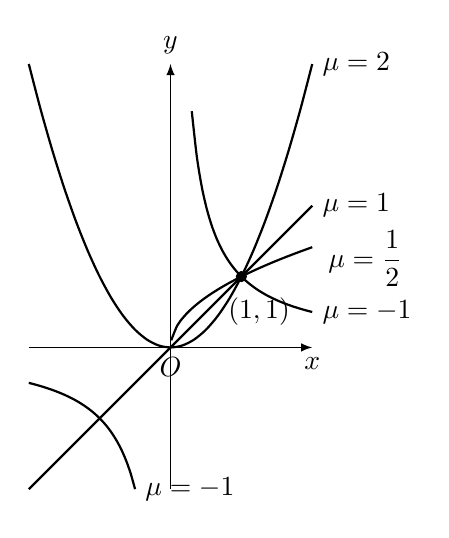
\begin{tikzpicture}[scale=0.9]
        \draw[-latex](-2,0) -- (2,0) node[below]{$x$};
        \draw[-latex](0,-2) -- (0,4) node[above]{$y$};
        \draw[black, thick, smooth, domain=0.3:2] plot (\x,1/\x) node[right]{$\mu =-1$};
        \draw[black, thick, smooth, domain=-2:-0.5] plot (\x,1/\x) node[right]{$\mu =-1$};
        \draw[black, thick, smooth, domain=0.01:2] plot (\x, {sqrt(\x)});
        \filldraw[black] (2.75,1.25) node {$\mu =\dfrac{1}{2}$};
        \draw[black, thick, smooth, domain=-2:2] plot (\x,\x) node[right]{$\mu =1$};
        \draw[black, thick, smooth, domain=-2:2] plot (\x, {\x*\x}) node[right]{$\mu =2$};
        \filldraw[black] (0,0) node[below]{$O$};
        \filldraw[black] (1,1) circle (2pt) node at(1.25,0.5){$(1,1)$};
    \end{tikzpicture}
\end{center}

\subsubsection{كۆرسەتكۈچلۈك فۇنكسىيە}\par\bigskip%
$y=a^x(a>0,a\neq 1)$
\begin{center}
    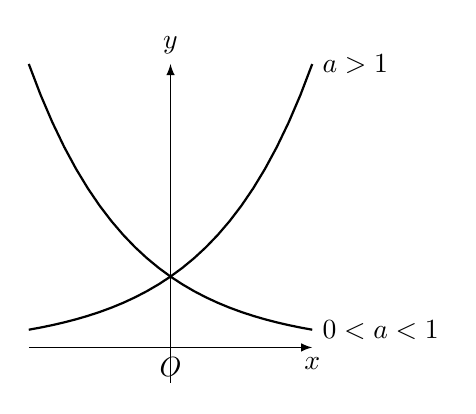
\begin{tikzpicture}[scale=0.9]
        \draw[-latex](-2,0) -- (2,0) node[below]{$x$};
        \draw[-latex](0,-0.5) -- (0,4) node[above]{$y$};
        \draw[black, thick, domain=-2:2] plot (\x,{pow(1/2,\x)}) node[right]{$0<a<1$};
        \draw[black, thick, domain=-2:2] plot (\x,{pow(2,\x)}) node[right]{$a>1$};
        \filldraw[black] (0,0) node[below]{$O$};
    \end{tikzpicture}
\end{center}

\subsubsection{لوگارىفمىلىق فۇنكسىيە}\par\bigskip
$y=log_ax(a>0,a\neq 1)$
\begin{center}
    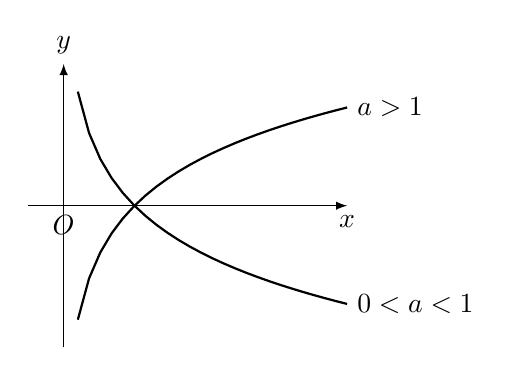
\begin{tikzpicture}[scale=0.9]
        \draw[-latex](-0.5,0) -- (4,0) node[below]{$x$};
        \draw[-latex](0,-2) -- (0,2) node[above]{$y$};
        \draw[black, thick, domain=0.2:4] plot (\x,{ln(1/\x)}) node[right]{$0<a<1$};
        \draw[black, thick, domain=0.2:4] plot (\x,{ln(\x)}) node[right]{$a>1$};
        \filldraw[black] (0,0) node[below]{$O$};
    \end{tikzpicture}
\end{center}

\subsubsection{ترىگونومېتىرىيەلىك فۇنكسىيە}\par\bigskip
سىنوس فۇنكىسىيەسى:
\begin{center}
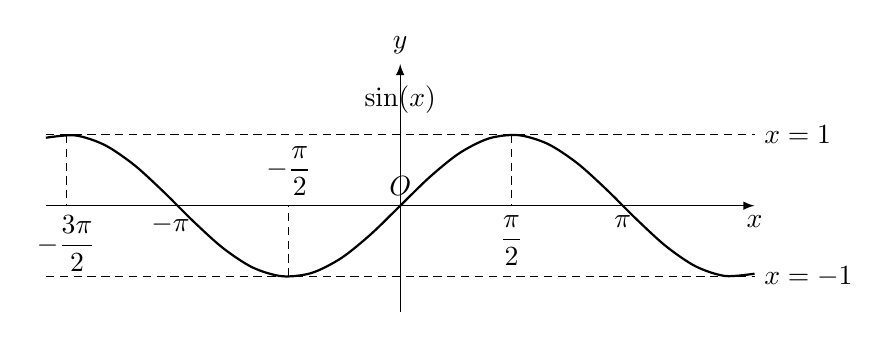
\begin{tikzpicture}[scale=0.9]
    \draw[-latex](-5,0) -- (5,0) node[below]{$x$};
    \draw[-latex](0,-1.5) -- (0,2) node[above]{$y$};
    \draw[black, thick, smooth, domain=-5:5] plot (\x,{sin(\x r)}) node at (0,1.5){$\sin(x)$};
    \draw[black, densely dashed](-5,1) -- (5,1) node[right]{$x=1$};
    \draw[black, densely dashed](-5,-1) -- (5,-1) node[right]{$x=-1$};
    \draw[black, densely dashed](-pi/2*3,1) -- (-pi/2*3,0) node[below]{$-\dfrac{3\pi}{2}$};
    \draw[black, densely dashed](-pi/2,-1) -- (-pi/2,0) node[above]{$-\dfrac{\pi}{2}$};
    \draw[black, densely dashed](pi/2,1) -- (pi/2,0) node[below]{$\dfrac{\pi}{2}$};
    \draw[black](0,0) -- (0,0) node[above]{$O$};
    \filldraw[black] (-pi-0.1,0) node[below]{$-\pi$};
    \filldraw[black] (pi,0) node[below]{$\pi$};
\end{tikzpicture}
\end{center}
كوسىنۇس فۇنكسىيەسى:
\begin{center}
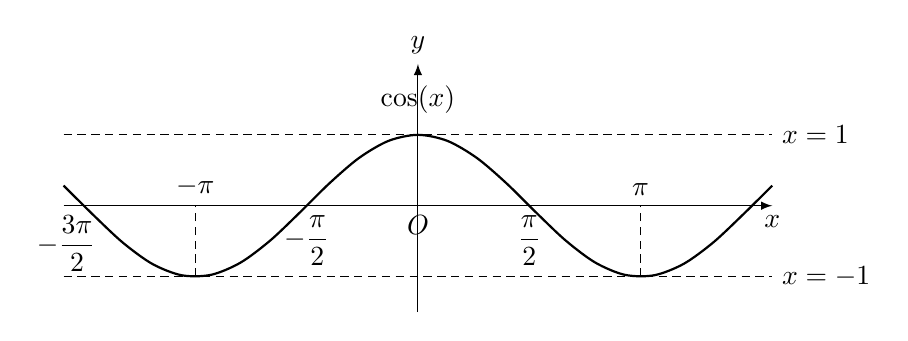
\begin{tikzpicture}[scale=0.9]
    \draw[-latex](-5,0) -- (5,0) node[below]{$x$};
    \draw[-latex](0,-1.5) -- (0,2) node[above]{$y$};
    \draw[black, thick, smooth, domain=-5:5] plot (\x,{cos(\x r)}) node at (0,1.5){$\cos(x)$};
    \draw[black, densely dashed](-5,1) -- (5,1) node[right]{$x=1$};
    \draw[black, densely dashed](-5,-1) -- (5,-1) node[right]{$x=-1$};
    \draw[black, densely dashed](-pi,-1) -- (-pi,0) node[above]{$-\pi$};
    \draw[black, densely dashed](pi,-1) -- (pi,0) node[above]{$\pi$};
    \filldraw[black] (0,0) node[below]{$O$};
    \filldraw[black] (-pi/2*3-0.25,0) node[below]{$-\dfrac{3\pi}{2}$};
    \filldraw[black] (-pi/2,0) node[below]{$-\dfrac{\pi}{2}$};
    \filldraw[black] (pi/2,0) node[below]{$\dfrac{\pi}{2}$};
\end{tikzpicture}
\end{center}
تانگېنىس فۇنكىسيەسى:
\begin{center}
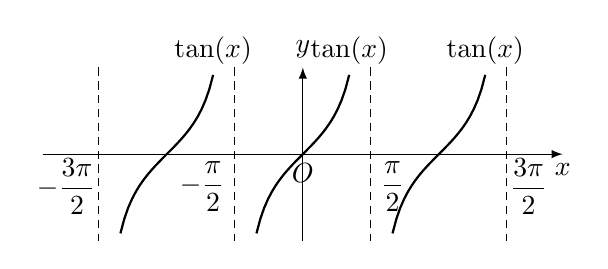
\begin{tikzpicture}[scale=0.55]
        \draw[-latex](-6,0) -- (6,0) node[below]{$x$};
        \draw[-latex](0,-2) -- (0,2) node[above]{$y$};
        \draw[black, thick, domain=-pi/2+0.5:pi/2-0.5] plot (\x,{tan(\x r)}) node[above]{$\tan(x)$};
        \draw[black, densely dashed](pi/2,2) -- (pi/2,-2);
        \draw[black, densely dashed](-pi/2,2) -- (-pi/2,-2);
        \draw[black, thick, domain=-pi/2*3+0.5:-pi/2-0.5] plot (\x,{tan(\x r)}) node[above]{$\tan(x)$};
        \draw[black, densely dashed](pi/2*3,2) -- (pi/2*3,-2);
        \draw[black, thick, domain=pi/2+0.5:pi/2*3-0.5] plot (\x,{tan(\x r)}) node[above]{$\tan(x)$};
        \draw[black, densely dashed](-pi/2*3,2) -- (-pi/2*3,-2);
        \filldraw[black] (0,0) node[below]{$O$};
        \filldraw[black] (pi/2+0.5,-0.75) node{$\dfrac{\pi}{2}$};
        \filldraw[black] (-pi/2-0.75,-0.75) node{$-\dfrac{\pi}{2}$};
        \filldraw[black] (pi/2*3+0.5,-0.75) node{$\dfrac{3\pi}{2}$};
        \filldraw[black] (-pi/2*3-0.75,-0.75) node{$-\dfrac{3\pi}{2}$};
    \end{tikzpicture}
\end{center}
كوتانگېنىس فۇنكسيەسى:
\begin{center}
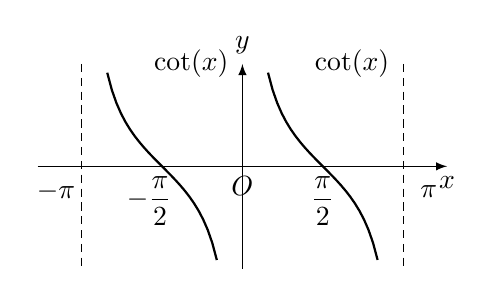
\begin{tikzpicture}[scale=0.65]
        \draw[-latex](-4,0) -- (4,0) node[below]{$x$};
        \draw[-latex](0,-2) -- (0,2) node[above]{$y$};
        \draw[black, thick, domain=0.5:pi-0.5] plot (\x,{cot(\x r)}) node at(pi-1,2){$\cot(x)$};
        \draw[black, densely dashed](pi,2) -- (pi,-2);
        \draw[black, thick, domain=-0.5:-pi+0.5] plot (\x,{cot(\x r)}) node at(-1,2){$\cot(x)$};
        \draw[black, densely dashed](-pi,2) -- (-pi,-2);
        \filldraw[black] (0,0) node[below]{$O$};
        \filldraw[black] (pi/2,0) node[below]{$\dfrac{\pi}{2}$};
        \filldraw[black] (pi+0.5,-0.5) node{$\pi$};
        \filldraw[black] (-pi/2-0.25,0) node[below]{$-\dfrac{\pi}{2}$};
        \filldraw[black] (-pi-0.5,-0.5) node{$-\pi$};
    \end{tikzpicture}
\end{center}

\subsubsection{تەتۈر ترىگونومېتىرىيەلىك فۇنكسىيە}\par\bigskip

تولۇقلىنىۋاتىدۇ...

\subsection{ترىگونومېتىرىيەلىك فۇنكسىيەلەر فورمۇلاسى}
يىغىندى:\\
\begin{align*}
    \sin \alpha \cos \beta & =\frac{1}{2}[\sin (\alpha+\beta)+\sin(\alpha-\beta)]  \\[7pt]
    \cos \alpha \sin \beta & =\frac{1}{2}[\sin (\alpha+\beta)-\sin(\alpha-\beta)]  \\[7pt]
    \cos \alpha \cos \beta & =\frac{1}{2}[\cos (\alpha+\beta)+\cos(\alpha-\beta)]  \\[7pt]
    \sin \alpha \sin \beta & =-\frac{1}{2}[\cos (\alpha+\beta)-\cos(\alpha-\beta)]
\end{align*}
كۆپەيمە:
\begin{align*}
    \sin\alpha+\sin\beta & =2\sin\frac{\alpha+\beta}{2}\cos\frac{\alpha-\beta}{2}  \\[7pt]
    \sin\alpha-\sin\beta & =2\cos\frac{\alpha+\beta}{2}\sin\frac{\alpha-\beta}{2}  \\[7pt]
    \cos\alpha+\cos\beta & =2\cos\frac{\alpha+\beta}{2}\cos\frac{\alpha-\beta}{2}  \\[7pt]
    \cos\alpha-\cos\beta & =-2\sin\frac{\alpha+\beta}{2}\sin\frac{\alpha-\beta}{2} \\[7pt]
    \tan\alpha+\tan\beta & =\frac{\sin (\alpha+\beta)}{\cos\alpha\cdot\cos \beta}
\end{align*}

بىرلىك:\\
\begin{align*}\label{gyhgs}
    \sin^2 x+\cos^2x  & =1 \\[7pt]
    \sec^2 x-\tan^2x  & =1 \\[7pt]
    \cosh^2x-\sinh^2x & =1
\end{align*}
يېرىم بۇلۇڭ:\\
\begin{align*}
    \sin^2x & =\frac{1}{2}(1-\cos 2x)                                                        \\[7pt]
    \cos^2x & =\frac{1}{2}(1+\cos 2x)                                                        \\[7pt]
    \tan^2x & =\frac{1-\cos 2x}{1+\cos 2x}                                                   \\[7pt]
    \sin x  & =2\sin\frac{x}{2}\cos\frac{x}{2}                                               \\[7pt]
    \cos x  & =2\cos^2\frac{x}{2}-1=1-2\sin^2\frac{x}{2}=\cos^2\frac{x}{2}-\sin^2\frac{x}{2} \\[7pt]
    \tan x  & =\frac{2\tan(x/2)}{1-\tan^2(x/2)}
\end{align*}

\subsection{ھاسىلە فورمۇلاسى}
\begin{multicols}{3}
    \begin{equation*}
        \left( C\right)'=0
    \end{equation*}
    \begin{equation*}
        \left( x^{\mu}\right)'=\mu x^{\mu-1}
    \end{equation*}
    \begin{equation*}
        \left( \sin x\right)'=\cos x
    \end{equation*}
    \begin{equation*}
        \left( \cos x\right)'=-\sin x
    \end{equation*}
    \begin{equation*}
        \left( \tan x\right)'=\sec^2 x
    \end{equation*}
    \begin{equation*}
        \left( \cot x\right)'=-\csc^2 x
    \end{equation*}
    \begin{equation*}
        \left( \sec x\right)'=\sec x\cdot\tan x
    \end{equation*}
    \begin{equation*}
        \left( \csc x\right)'=-\csc x\cdot\tan x
    \end{equation*}
    \begin{equation*}
        \left( a^x\right)'=a^x\ln a\ (a>0,a\neq1)
    \end{equation*}
    \begin{equation*}
        \left( \log_{a}x\right)'=\frac{1}{x\cdot\ln a}\ (a>0,a\neq1)
    \end{equation*}
    \begin{equation*}
        \left( \arcsin x\right)'=\frac{1}{\sqrt{1-x^2}}
    \end{equation*}
    \begin{equation*}
        \left( \arccos x\right)'=-\frac{1}{\sqrt{1-x^2}}
    \end{equation*}
    \begin{equation*}
        \left( \arctan x\right)'=\frac{1}{1+x^2}
    \end{equation*}
    \begin{equation*}
        \left( \mathrm{arccot}\, x\right)'=-\frac{1}{1+x^2}
    \end{equation*}
\end{multicols}

\subsection{ئىنتېگىرال فورمۇلاسى}
\begin{align*}
     & \int x^\mu\,\mathrm{d}x=\frac{x^{\mu+1}}{\mu+1}+C\ (\mu\neq-1)                                                         \\[7pt]
     & \int \frac{1}{x}\,\mathrm{d}x=\ln|x|+C                                                                                 \\[7pt]
     & \int\frac{\mathrm{d}x}{1+x^2}=\arctan x+C                                                                              \\[7pt]
     & \int\frac{\mathrm{d}x}{\sqrt{1-x^2}}=\arcsin x+C_1=-\arccos x+C_2                                                      \\[7pt]
     & \int \sin x\,\mathrm{d}x=-\cos x+C                                                                                     \\[7pt]
     & \int\cos x \,\mathrm{d}x=\sin x +C                                                                                     \\[7pt]
     & \int\tan x\,\mathrm{d}x=-\ln |\cos x|+C                                                                                \\[7pt]
     & \int\cot x\,\mathrm{d}x=\ln |\sin x|+C                                                                                 \\[7pt]
     & \int\csc x\,\mathrm{d}x=\int\frac{1}{\sin{x}}\,\mathrm{d}x=\frac{1}{2}
    \ln{\left|\frac{1-\cos{x}}{1+\cos{x}}\right|}+C=\ln{\left|\tan{\frac{x}{2}}\right|}+C=\ln{\left|\csc{x}-\cot{x}\right|}+C \\[7pt]
     & \int\sec x\,\mathrm{d}x=\int\frac{1}{\cos{x}}\,\mathrm{d}x=\frac{1}{2}
    \ln{\left|\frac{1+\sin{x}}{1-\sin{x}}\right|}+C=\ln{\left|\sec{x}+\tan{x}\right|}+C                                       \\[7pt]
     & \int\sec^2 x\,\mathrm{d}x=\tan x +C                                                                                    \\[7pt]
     & \int \csc^2 x\,\mathrm{d}x=-\cot x +C                                                                                  \\[7pt]
     & \int \sec x\cdot\tan x \,\mathrm{d}x=\sec x+C                                                                          \\[7pt]
     & \int\csc x \cdot\cot x \,\mathrm{d}x=-\csc x+C                                                                         \\[7pt]
     & \int \mathrm{e}^x \,\mathrm{d}x=\mathrm{e}^x+C                                                                         \\[7pt]
     & \int a^x\,\mathrm{d}x=\frac{a^x}{\ln a}+C                                                                              \\[7pt]
     & \int \sinh x\,\mathrm{d}x=\cosh x+C                                                                                    \\[7pt]
     & \int \cosh x\,\mathrm{d}x=\sinh x+C                                                                                    \\[7pt]
     & \int \frac{1}{a^2+x^2}\,\mathrm{d}x=\frac{1}{a}\arctan\frac{x}{a}+C                                                    \\[7pt]
     & \int \frac{1}{a^2-x^2}\,\mathrm{d}x=\frac{1}{2a}\ln \left|\frac{a+x}{a-x}\right|+C                                     \\[7pt]
     & \int \frac{1}{\sqrt{a^2-x^2}}\,\mathrm{d}x=\arcsin\frac{x}{a}+C                                                        \\[7pt]
     & \int \frac{1}{\sqrt{x^2\pm a^2}}\,\mathrm{d}x=\ln \left|x+\sqrt{x^2\pm a^2}\right|+C
\end{align*}

\section{سانلار ئارقىمۇ ئارقىلىقى}
\subsection{تەڭ ئايرىمىلىق سانلار ئارقىمۇ ئارقىلىقى}

\subsection{تەڭ نىسبەتلىك سانلار ئارقىمۇ ئارقىلىقى}

\subsection{سانلار قاتارى}

\subsection{سانلار قاتارى يىغىندىسى}
\begin{english}
\begin{enumerate}
    \item $\sum_{k=1}^nk=1+2+\cdots+n=\dfrac{n(n+1)}{2}$
    \item $\sum_{k=1}^nk^2=1^2+2^2+\cdots+n^2=\dfrac{n(n+1)(2n+1)}{6}$
    \item $\sum_{k=1}^n\dfrac{1}{k(k+1)}=\dfrac{1}{1\times 2}+\dfrac{1}{2\times 3}+\cdots+\dfrac{1}{n(n+1)}=\dfrac{n}{n+1}$
\end{enumerate}
\end{english}

دەرىجە فۇنكسىيەسىگە نىسبەتەن ئوخشاش بولمىغان دەرىجە ئاستىدىكى ئوخشاش مونوتونلۇققا ئاساسەن ئەڭ قىممەتنى تەتقىق قىلىشقا بولىدۇ.
\newpage
\mychapter{فۇنكسىيە ۋە لىمىت نەزەرىيىسى}
\section{فۇنكىسىيە}
فۇنكسىيەنىڭ ئېنىقلىمىسى ئادەتتە ئەنئەنىۋى ئېنىقلىما ۋە زامانىۋى ئېنىقلىما دەپ ئىككىگە بۆلىنىدۇ. باياننىڭ ئۇقۇمىنىڭ باشلىنىش نۇقتىسى باشقىچە بولغاندىن باشقا ، فۇنكىسىيەنىڭ ئىككى ئېنىقلىمىسى ئاساسەن ئوخشاش. ئەنئەنىۋى ئېنىقلىما ھەرىكەت ئۆزگىرىشى نۇقتىسىدىن باشلىنىدۇ. ، زامانىۋى ئېنىقلىما بولسا توپلام ۋە ئەكىس ئېتىش نۇقتىسىدىن باشلىنىدۇ.

\begin{MyDefinition}{فۇنكىسىيەنىڭ ئېنىقلىمىسى}{}
 خالىغان توپلام $A$ دىكى ئېلمىنىت $x$ گە نىسبەتەن، ماسلىق مۇناسىۋىتى $f$ مەۋجۇت بولۇپ، بۇ $x$ گە تەسىر قىلىغاندىن كىيىن ئېرىشكەن توپلام $B$ نىڭ ئېلمىنتى $y$ بولسا، ئۇنداقتا $f(x)$ بولسا توپلام $A$ دىن توپلام $B$ غا بولغان ئەكىس ئېتىش ھېساپلىنىدۇ. بۇنىڭدا $y$ بولسا $x$ نىڭ فۇنكىسىيەسى دېيىلىدۇ. بۇنى 
 $$x:\rightarrow y \Leftrightarrow y=f(x)$$
 ئارقىلىق خاتېرلەشكە بولىدۇ.
\end{MyDefinition}
فۇنكىسىيە ئۇقۇمى ئۈچ دائىرىنى ئۆز ئىچىگە ئالىدۇ: ئېنىقلىما ساھەسى $A$ ، قىممەت دائىرىسى $B$ ۋە مۇناسىۋەت ئىپادىسى $f$

\section{سانلار قاتارى}
بۇ بۆلەك تولۇقلىنىلىۋاتىدۇ.
\subsection{تەڭ ئايرىمىلىق سانلار ئارقىمۇ-ئارقىلىقى}
\subsection{تەڭ نىسبەتلىك سانلار ئارقىمۇ-ئارقىلىقى}
\subsection{سانلار قاتارى}

\section{لىمىت}
بۇ بۆلەك تولۇقلىنىلىۋاتىدۇ.
\subsection{لىمىت ۋە ئۇنىڭ خۇسۇسىيەتلىرى}
\subsection{سانلار قاتارى لىمىتى}
\subsection{فۇنكىسىيە لىمىتى}
\subsection{سانلار قاتارى ۋە فۇنكىسىيە لىمىتى}

\section{فۇنكىسىيە ئۈزلۈكسىزلىكى}
بۇ بۆلەك تولۇقلىنىلىۋاتىدۇ.
\subsection{فۇنكىسىيە مونوتونلىقى}
\subsection{فۇنكىسىيە ئۈزۈك نۇقتىسى}

\newpage
\mychapter{دىففېرېنسىيال ۋە ئىنتېگرال}
\par\bigskip
\begin{tcolorbox}
	\textcolor{blue}{\textbf{بۇ باپتىكى مۇھېم نۇقتىلار:}}
دىففېرېنسىيال ۋە ئىنتېگرال ماتىماتىكا پېنىدىكى ئەڭ يادرولۇق بىلىم نۇقتىسىنىڭ بىرى، شۇنداقلا ئۇ فىزىكا ئىلمىنىڭ ئاساسى. بۇ باپتا ھاسىلە ئۇقۇمىدىن باشلاپ دىففېرېنسىيال ۋە ئىنتېگرالنىڭ ئەمەلىي قوللىنىشىغىچە بولغان مەزمۇنلار خاتىرلىنىدۇ. بۇ باپتا يەنە دىففېرېنسىيال ۋە ئىنتېگرالغا ئائىت ھېسابلاشلار، تېئورېمىلار چۈشەندۈرىلىدۇ. بۇنىڭدىن سىرت دىففېرېنسىيال ۋە ئىنتېگرالنىڭ ماھىيىتى ۋە قوللىنىلىشىغا دائىر ئەمەلىي مىساللار تونۇشتۇرلىدۇ.
\end{tcolorbox}

\section{ھاسىلە ئۇقۇمى}
تىزلىك ئۇقۇمى ھەممە كىشىگە ئەڭ تونۇش بولسا كىرەك، مەسىلەن ماشىنا تىزلىكى $60 km/h$ دىگەندەك. بۇ يەردىكى  $60 km/h$ ئەمەلىيەتتە  $16.67 m/s$ بىلەن ئوخشاش. يەنى 1 سېكۇنىتتا 16.67 مىتېر يۆتكىلىدۇ دىگەنلىك. تىزلىك قانداق قىلىپ ماڭغان يۆتكىلىشكە ئايلاندى؟ ماڭغان يۆتكىلىش قانداق قىلىپ تىزلىكنى مەۋجۇت قىلدى؟ جىسىم مەلۇم تىزلىككە يىتىش ئۈچۈن تىنىچ ھالەتتىن قوزغالسا، ئۇ نىشان تىزلىككە يەتكۈچە قانداق قىلىپ تىزلىنىشنى مەۋجۇت قىلدى؟ بۇنداق فىزىكىلىق ھادىسىلەرنى تەتقىق قىلىشتا ھاسىلىگە تايانماي بولمايدۇ.
\subsection{فۇنكىسىيە ھاسىلىسى}
\subsection{يۇقچى دەرىجىلىك ھاسىلە}

\section{دىففېرېنسىيال}
\begin{figure}[htp]
  \centering
  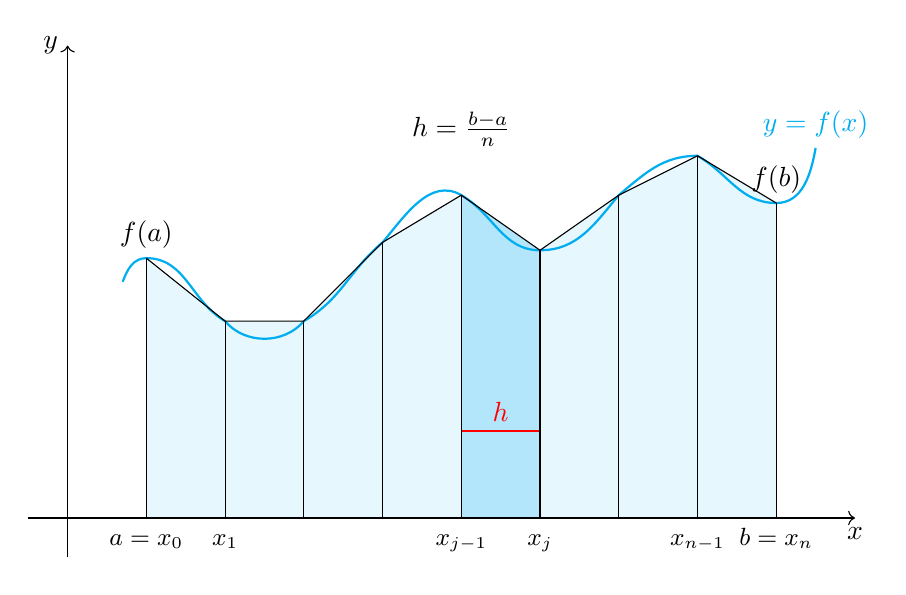
\begin{tikzpicture}
    \coordinate (p1) at (0.7,3); 
    \coordinate (p2) at (1,3.3);
    \coordinate (p3) at (2,2.5); 
    \coordinate (p4) at (3,2.5);
    \coordinate (p5) at (4,3.5); 
    \coordinate (p6) at (5,4.1);
    \coordinate (p7) at (6,3.4); 
    \coordinate (p8) at (7,4.1);
    \coordinate (p9) at (8,4.6); 
    \coordinate (p10) at (9,4);
    \coordinate (p11) at (9.5,4.7);

    % The cyan background
    \fill[cyan!10] (p2|-0,0) -- (p2) -- (p3) -- (p4) -- (p5) -- (p6)
    -- (p7) -- (p8) -- (p9) -- (p10) -- (p10|-0,0) -- cycle;
    % the dark cyan stripe
    \fill[cyan!30] (p6|-0,0) -- (p6) -- (p7) -- (p7|-0,0) -- cycle;
    % the curve
    \draw[thick,cyan] (p1) to[out=70,in=180] (p2) to[out=0,in=150]
    (p3) to[out=-50,in=230] (p4) to[out=30,in=220] (p5)
    to[out=50,in=150] (p6) to[out=-30,in=180] (p7) to[out=0,in=230]
    (p8) to[out=40,in=180] (p9) to[out=-30,in=180] (p10)
    to[out=0,in=260] (p11);
    % the broken line connecting points on the curve
    \draw (p2) -- (p3) -- (p4) -- (p5) -- (p6) -- (p7) -- (p8) -- (p9)
    -- (p10);

    % the h line
    \draw[red,thick] ($(p6) + (0.0, -3.0)$) --
    node[above,red]{$h$}($(p6) + (1.0, -3.0)$);
    \node[above,yshift=0.5cm,text=black] at (p6) {$h=\frac{b-a}{n}$};
        
    % vertical lines and labels
    \foreach \n/\texto in { 2/{a=x_0}, 3/{x_1}, 4/{}, 5/{},
      6/{x_{j-1}}, 7/{x_j}, 8/{}, 9/{x_{n-1}}, 10/{b=x_n} } { \draw
      (p\n|-0,0) -- (p\n); \node[below,text height=1.5ex,text
      depth=1ex,font=\small] at (p\n|-0,0) {$\texto$}; }
        
    % The axes
    \draw[->] (-0.5,0) -- (10,0) coordinate (x axis); \draw[->]
    (0,-0.5) -- (0,6) coordinate (y axis);
    % labels for the axes
    \node[below] at (x axis) {$x$}; \node[left] at (y axis) {$y$};
    % label for the function
    \node[above,text=cyan] at (p11) {$y=f(x)$};

    % label for the f(a)和f(b)
    \node[above,text=black] at (p2) {$f(a)$}; \node[above,text=black]
    at (p10) {$f(b)$};
  \end{tikzpicture}
  \caption{دېففېرىرېنسىئال}\label{fig-integrate}
\end{figure}
\subsection{فۇنكىسىيە دىففېرېنسىيالى}
\subsection{ھاسىلە فورمۇلىسى}


\section{دىففېرېنسىيال تېئورمىسى}
\subsection{فېرمات تېئورمىسى}
\subsection{لور تېئورمىسى}
\subsection{لاگرانج تېئورمىسى}
\subsection{كوشى تېئرمىسى}
\subsection{دىففېرېنسىيال ئوتتۇرا قىممەت تېئورمىسى}

\section{تەيلېر يېيىلمىسى}
\subsection{تەيلېر يىيېلمىسى}
\subsection{تەيلېر فورمۇلىسى}

\section{فۇنكىسىيە خۇسۇسىيىتى}
\subsection{فۇنكىسىيە يىلتېزى}
\subsection{فۇنكىسىيە مونوتون رايونى}
\subsection{فۇنكىسىيە ئېكىستېرمۇم قىممىتى}
\subsection{فۇنكىسىيە كۆپۈنگۈ ۋە پېتىنقى قىسمى}
\subsection{فۇنكىسىيە بۇرۇلۇش نۇقتىسى}

\section{ياي دىففېرېنسىيالى}
\subsection{ياي دىففېرېنسىيالى}
\subsection{ئەگرىلىك}
\subsection{ئەگرىلىك رادېئۇس}

\newpage
\mychapter{ئېنىق ئىنتېگرال ۋە ئېنىقسىز ئىنتېگرال}

\section{ئېنىق ئىنتېگرال}
\subsection{ئۇقۇم ۋە خۇسۇسىيەت}
\subsection{ئالماشتۇرۇش ئۇسۇلى}
\subsubsection{بىرىنچى خىل ئالماشتۇرۇش}
\subsubsection{ئىككىنچى خىل ئالماشتۇرۇش}
\subsection{قەدەملەش ئۇسۇلى}
\subsection{راتسىيونال فۇنكىسىيە ئىنتېگرالى}

\section{ئېنىقسىز ئىنتېگرال}
\subsection{ئۇقۇم ۋە خۇسۇسىيەت}
\subsection{ھېساپلاش}
\subsection{نىيۇتون-لېبرېنتىس فورمۇلسى}
\subsection{غەيرى ئىنتېگرال}

\section{ئىنتېگرال قوللىنىلىشى}
\subsection{يۈز}
\subsection{ھەجىم}
\subsection{ئوتتۇرىچە قىممەت}
\subsection{ئوزۇنلۇق}

\subsection{ئىنتېگرال جەدۋىلى}
\newpage
\mychapter{كۆپ ئۆزگەرگۈچىلىك فۇنكسىيە}
بۇ باپ تولۇقلىنىلىۋاتىدۇ.
\section{ئاساسىي بىلىم}
\subsection{تەكشىلىك ۋە نۇقتا}
\subsection{لىمىت}
\subsection{خۇسۇسىي ھاسىلە}
\subsection{تولۇق ھاسىلە}
\subsection{ھاسىلە ئۈزلۈكسىزلىكى}
\section{كۆپ ئۆزگەرگۈچىلىك فۇنكسىيە ھاسىلىسى}
\subsection{زەنجىر قائىدىسى}
\subsection{يوشۇرۇن فۇنكسىيە مەۋجۇتلىقى}

\section{كۆپ ئۆزگەرگۈچىلىك فۇنكسىيە ئېكسترىمۇم }
\subsection{ئاساسىي ئۇقۇم}
\subsection{شەرتسىز ئېكستىرىمۇم}
\subsection{شەرتلىك ئېكسىترىمۇم}


\newpage
\mychapter{كۆپ ئۆزگەرگۈچىلىك فۇنكسىيە ئىنتېگرالى}

\section{قوش قات ئىنتېگرال}
\subsection{ئاساسىي ئۇقۇم}
\subsection{ھېساپلاش}
\subsection{ئەمەلىي قوللىنىلىشى}

\section{ئۈچ قات ئىنتېگرال}
\subsection{ئاساسىي ئۇقۇم}
\subsection{ھېساپلاش}
\subsection{ئەمەلىي قوللىنىلىشى}

\section{بىرىنچى ئەگرى سىزىق ئىتېگرال}
\subsection{ئاساسىي ئۇقۇم}
\subsection{ھېساپلاش}
\subsection{ئەمەلىي قوللىنىلىشى}

\section{ئىككىنچى ئەگرى سىزىق ئىتېگرال}
\subsection{ئاساسىي ئۇقۇم}
\subsection{ھېساپلاش}
\subsection{گىرىن فورمۇلىسى}
\subsection{ئەمەلىي قوللىنىلىشى}

\section{بىرىنچى سىرت ئىتېگرال}
\subsection{ئاساسىي ئۇقۇم}
\subsection{ھېساپلاش}
\subsection{ئەمەلىي قوللىنىلىشى}


\section{ئىككىنچى سىرت ئىتېگرال}
\subsection{ئاساسىي ئۇقۇم}
\subsection{گائۇس فورمۇلىسى}
\subsection{ھېساپلاش}

\section{ئەمەلىي قوللىنىلىشى}
\subsection{ئېغىرلىق ۋە شەكىل مەركىزىى}
\subsection{ئايلىنىش ئېنېرتسىيەسى}

\newpage
\mychapter{چەكسىز قاتار}
\par\bigskip
\begin{tcolorbox}
\textcolor{blue}{\textbf{بۇ باپتىكى مۇھېم نۇقتىلار:}}
مۇسبەت قاتارنىڭ يىغىلىشچانلىقىنى سېلىشتۇرۇپ ئېنىقلاش ئۇسۇلى، نىسبەت قىممىتى ئېنىقلاش ئۇسۇلى، يىلتىز قىممىتىنى ئېنىقلاش ئۇسۇلى، گىرەلەشمە قاتارنىڭ لېبنىز ئېنىقلاش ئۇسۇلى. قىيىن نۇقتا خالىغان قاتارنىڭ ئابېل پەرقلەندۈرۈش ئۇسۇلى ۋە دىرىكلېي پەرقلەندۈرۈش ئۇسۇلى قاتارلىقلار.
\end{tcolorbox}

\section{ئاساسىي ئۇقۇملار}
ھەرقانداق سانلار ئارقىمۇ ئارقىلىقى 
$\{a_1,a_2,...,a_n,a_{n+1},...\}$
غا نىسبەتەن، ئۇنىڭ خالىغان ئېلمنىتلىرىنىڭ چېكى بولسا، بىز بۇنى \textbf{چېگرىلانغان} دەپ ئاتايمىز. يەنى تۆۋەندىكىدەك ئىپادە قۇرىلىدۇ:
$$
A_k \le a_{k+n} \le B_k, (k=1,2,....,n=1,2,..., n>k)
$$
دېمەك يۇقىرىدىكى $A_k,B_k$ لار بۇ سانلارنىڭ \textbf{ئېنىق چېكى} دەپ ئاتىلىدۇ.\\بۇنىڭدا $A_k$ ئېنىق ئاستا چېكى دىيىلىدۇ ھەم
$A_k = inf \{a_{k+n}\},(k=1,2,....,n=1,2,..., n>k)$
قىلىپ خاتىرلىنىدۇ، ئوخشاشلا $B_k$ ئېنىق ئۈستى چېكى دىيىلىدۇ ھەم
$B_k = sup \{a_{k+n}\},(k=1,2,....,n=1,2,..., n>k)$
قىلىپ خاتىرلىنىدۇ.
بۇ يەردىكى ئېنىق چېكى مۇقىم ئەمەس بولۇپ، شۇڭا ئىندېكسى $k$ قوشۇپ يېزىلىدۇ. بۇ خۇددى مەلۇم بىر ساننىڭ بەشتىن كىچىك بولسا، ئۇ ساننىڭ ئالتىدىنمۇ كىچىك، يەتتىدىنمۇ كىچىك، ... ، بولىدىغانلىقى بىلەن ئوخشاش مەنىدە.\\
ئەگەر يۇقارقى سانلار ئارقىمۇ ئارقىلىقى يىغىلسا، ئۇنىڭ لىمىتى چوقۇم مەۋجۇت بولىدۇ. شۇنىڭ بىلەن ئۇنىڭ لىمىتى ۋە ئېنىق چېكى ئوتتۇرىسىدا  مۇنداق مۇناسىۋەت ئىپادىسى قۇرىلىدۇ:
\begin{align*}
A = \lim_{k \to \infty}A_k = \lim_{k\to\infty} inf \{a_{k+n}\} \\
B = \lim_{k \to \infty}B_k = \lim_{k\to\infty} sup \{a_{k+n}\}
\end{align*}

دىمەك، بۇيەردىكى $A,B$ لار $\{a_1,a_2,...,a_n,a_{n+1},...\}$ نىڭ ئاستى لىمىتى ۋە ئۈستى لىمىتى دەپ ئاتىلىدۇ. شۇنىڭ بىلەن يىغىلىدىغان سانلار ئارقىمۇ ئارقىلىقى ۋە ئۇنىڭ چېگرىسى ئارىسىدىكى مۇناسىۋەت لىمىت بىلەن باغلانغان بولىدۇ.
\textcolor{red}{
سانلار ئارقىمۇ ئارقىلىقىنىڭ لىمىتى ۋە ئۇنىڭ ئاستى ئۈستى لىمىتلىرىنى ئارىلاشتۈرۋېتىشكە بولمايدۇ. ئاستى ئۈستى لىمىتلىرىنى مەۋجۇت بولسا سانلارنىڭ لىمىتى مەۋجۇت بولىشى ناتايىن.} مەسىلەن تۆۋەندىكى رەسىمدە:\\
\begin{figure}[htbp]
\begin{tikzpicture}
	\begin{axis}
		\addplot[color=red]{1/exp(x)};
		\legend{$e^{-x}$}
	\end{axis}
\end{tikzpicture}
\hskip 10pt
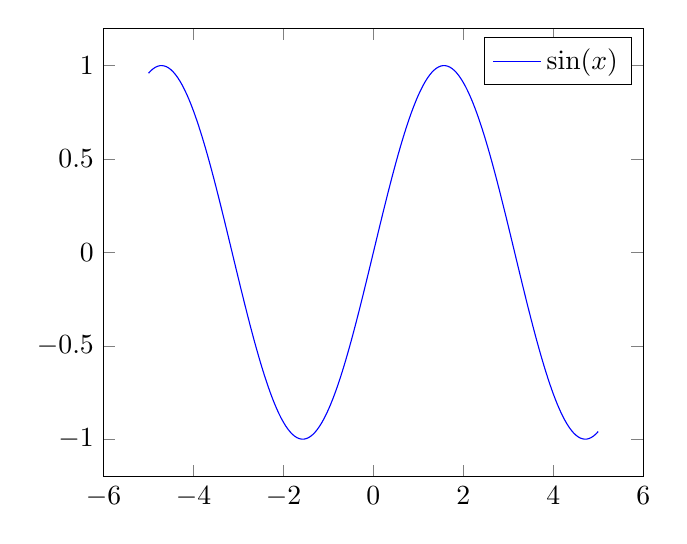
\begin{tikzpicture}
	\begin{axis}
		\addplot [blue,samples=201] {sin(deg(x))};
		\legend{$\sin(x)$}
	\end{axis}
\end{tikzpicture}
\end{figure}

سىنوس فۇنكىسىيەلىك سانلار ئارقىمۇ ئارىلىقىنىڭ لىمىتى يوق، ئۇنىڭ ئاستى ئۈستى چېكى بار، $1$ ۋە $-1$ دەل ئۇنىڭ ئاستى ئۈستى چېكى، شۇنداقلا ئۇنىڭ ئاستى ئۈستى لىمىتلىرى بار. ئوخشاشلا سول تەرەپتىكى رەسىمدىكىدەك، $e^{-x}$ فۇنكىسىيەلىك سانلار ئارقىمۇ ئارقىلىقىنىڭ ئاستى چېكى بار، ئاستى لىمىتى بار يەنى $0$ ، ئەمما ئۈستى لىمىتى يوق. شۇڭا ئۆزگەرگۈچى مىقدار $x$ چەكسىزلىككە يۈزلەنگەندە ئۇنىڭ لىمىتى بار، بۇ دەل ئۇنىڭ ئاستى لىمىتى.

\subsection{قاتار}
ئوتتۇرا مەكتەپ ماتېماتىكا دەرسىدە سانلار ئارقىمۇ ئارقىلىقى ھەققىدە مۇناسىۋەتلىك بىلىملەرنى دەسلەپ ئۆگىنىمىز. ئۇ ۋاقىتتا پەقەت چەكلىك ئەزالىق سانلار ئارقىمۇ ئارقىلىقى ئۈستىدە، يەنە كىلىپ تەڭ ئايرىمىلىق ۋە تەڭ نىسبەتلىك سانلار ئارقىمۇ ئارقىلىقى ئۈستىدىلا ئۆگىنىش ئېلىپ بېرىلاتتى. ئەمدىكى مەزمۇندا چەكسىز بولغان سانلار ئارقىمۇ ئارقىلىقى «قاتار» ئۈستىدە مۇلاھېزە ئېلىپ بارىمىز.
\par
ئالدىنقى مەزمۇنلاردا سانلار قاتارى ھەقتە مەزمۇنلار خاتېرلەنگەن ئىدى. بولۇپمۇ تەڭ ئايرىمىلىق   سانلار ئارقىمۇ-ئارقىلىقى ۋە تەڭ نىسبەتلىك سانلار ئارقىمۇ-ئارقىلىقى ئۈستىدە تەپسىلىي نۇقتىلار يېزىلدى. ئەمدى بۇ باپتا قاتار ئۇقۇمى بىلەن تونۇشۇپ چىقىمىز. قاتار دېگەن نۇرغۇنلىغان ئېلمىنتلارنىڭ يىغىندىسىدىن تەركىپ تاپقان ئىپادە بولۇپ، چەكسىز قاتار بولسا چەكسىز ئېلمىنتلار قاتارىنى كۆرسىتىدۇ.

\begin{MyDefinition}{قاتار}{}
خالىغان سانلار ئارقىمۇ-ئارقىلىقى $u_1,u_2,\cdots,u_n,\cdots$ نىڭ ئېلمىنىتلىرىنى قوشۇش ئەمىلى بىلەن ئۇلاپ يېزىپ ھاسىل بولغان ئىپادە ئىپادە چەكسىز قاتار دەپ ئاتىلىدۇ(قىسقارتىلىپ قاتار دېيىلىدۇ).ماتېماتىكىدا 
$$\sum\limits_{n=1}^\infty u_n=u_1+u_2+\cdots+u_n+\cdots$$
 قىلىپ خاتىرلىنىدۇ.
\end{MyDefinition}

	ئېنىقلىمىدىكى $u_n$ قاتارنىڭ \textbf{ئومۇمىي ئەزاسى} دەپ ئاتىلىدۇ. ئالدىنقى $n$ ئەزاسىنىڭ يىغىندىسى \textbf{قىسمەن يىغىندى} دەپ ئاتىلىدۇ، ھەم $S_n=u_1+u_2+\cdots+u_n$ قىلىپ خاتىرلىنىدۇ.

\paragraph{ئادەتتىكى ئەزالىق قاتار}
ئەگەر قاتارنىڭ ئومۇمىي ئەزاسى $u_n$ تۇراقلىق سان بولسا، بۇ خىلدىكى قاتارنىڭ ئادەتتىكى ئەزالىق قاتار دەپ ئاتايمىز. مەسىلەن: 
$
\sum_{n=1}^{\infty} = 1+2+...+n+.... ,\quad \sum_{n=1}^{\infty} = 1+\frac{1}{2}+\frac{1}{3}+...+\frac{1}{n}+...
$
ئادەتتىكى ئەزالىق قاتار ھېساپلىنىدۇ.

\subsection{قاتارنىڭ يىغىلىشچانلىقى ۋە خۇسۇسىيىتى}

\subsubsection{يىغىلىشچانلىقى}
ئەگەر قاتارنىڭ قىسمەن يىغىندىسى $S_n$ نىڭ لىمىتى مەۋجۇت بولسا، بۇ قاتار \textbf{يىغىلىدۇ} دەپ ئاتىلىدۇ. يەنى، ئەگەر $\lim\limits_{n\to\infty}S_n=S$، ئۇنداقتا $\sum\limits_{n=1}^\infty u_n$. 
ئەگەر قاتارنىڭ قىسمەن يىغىندىسى $S_n$ نىڭ لىمىتى مەۋجۇت بولمسا، ئۇنداقتا بۇ قاتار \textbf{يىراقلىشىشىدۇ} دەپ ئاتىلىدۇ.\\
قاتارنىڭ يىغىلىش ۋە يىراقلىىشىنىڭ يۈزەكى مەنىسى بولسا، يىغىلغاندا ئۇنىڭ يىغىندىسىنىڭ چېكى بار، يىراقلاشقاندا ئۇنىڭ يىغىندىسىنىڭ چېكى يوق.
\subsubsection{خۇسۇسىيىتى}
قاتارنىڭ ئېنىقلىمىسى ۋە يىغىلىشچانلىقىغا ئاساسەن تۆۋەندىكى بىرقانچە خۇسۇسىيەتلەرگە ئېرشەلەيمىز.
\begin{WhiteRule}{قاتار يىغىلىشىنىڭ زۆرۈر شەرتى}{}%
ئەگەر قاتار 
$\sum\limits_{n=1}^\infty u_n=u_1+u_2+\cdots+u_n+\cdots$
 يىغىلسا، ئۇنىڭ ئومۇمىي ئەزاسىنىڭ لىمىتى 
$\lim\limits_{n \to \infty}u_n = 0$
 چوقۇم مەۋجۇت ھەم نۆلگە تەڭ.
\end{WhiteRule}
بۇنىڭ سەۋەبىنى قاتارنىڭ قىسمەن يىغىندىسى $S_n$ دىن كۆرۈۋىلىشقا بولىدۇ.\\
ئېنىقلىمىغا ئاساسەن قاتار يىغىلسا ئۇنىڭ قىسمەن يىغىندىسىنىڭ لىمىتى بار ئىدى،
$S = \lim\limits_{n \to \infty}S_n$
 ھەم
$u_n = S_n - S_{n-1}$
شۇڭا 
$\lim\limits_{n \to \infty}u_n = \lim\limits_{n \to \infty}S_n - \lim\limits_{n \to \infty}S_{n-1} = S-S=0$.\\
\textcolor{red}{شۇنى ئەسكەرتىشكە تېگىشلىكى بۇ پەقەت زۆرۈر شەرت، يىتەرلىك شەرت ئەمەس}، شۇڭا ئومۇمىي ئەزانىڭ لىمىتى $0$ بولسا، قاتارنىڭ لىمىتى مەۋجۇت بولىشى ناتايىن. مەسىلەن تۆۋەندىكى قاتارنىڭ ئومۇمىي ئەزا لىمىتى بار يەنى 
$
\lim_{n \to \infty} \frac{1}{n} = 0
$
، ئەمما قاتار يىغىلمايدۇ
$$
\sum\limits_{n=1}^\infty u_n = 1+\frac{1}{2}+\frac{1}{3}+...+\frac{1}{n}+... = +\infty
$$

\begin{WhiteRule}{يىغىلىشچان قاتارنىڭ سىزىقلىق خۇسۇسىيتى}{}%
ئەگەر قاتار 
$\sum\limits_{n=1}^\infty u_n$
ۋە
$\sum\limits_{n=1}^\infty v_n$
يىغىلسا، ئۇلارنىڭ سىزىقلىق ھېساپلاشلىرى 
\begin{equation*}
\sum\limits_{n=1}^\infty (\alpha u_n \pm \beta v_n)
=\alpha\sum\limits_{n=1}^\infty \pm \beta \sum\limits_{n=1}^\infty v_n
\end{equation*}
ئوخشاشلا يىغىلىدۇ. بۇ يەردە $\alpha,\beta$ لار خالىغان ھەقىقىي سان.
\end{WhiteRule}
بۇ خۇسۇسىيتىگە ئىسپاتلاش ياكى چۈشەنچە بېرىلمەيدۇ، چۈنكى سىزىقلىق ئالگېبرادىكى ئىدىيە بويىچە تۇرقلىق سان بىلەن سزىقلىق ھېساپلاش ئېلپ بېرىلغان قاتارنىڭ خۇسۇسىيەتلىرى ئۆزگەرمەيدۇ.
\begin{WhiteRule}{يىغىلىشچان قاتارنىڭ تىرناق خۇسۇسىيتى}{}%
ئەگەر قاتار 
$\sum\limits_{n=1}^\infty u_n=u_1+u_2+\cdots+u_n+\cdots$
يىغىلسا، ئۇنىڭ ئومۇمىي ئەزالىرىنىڭ خالىغان يېرىگە خالىغان تىرناق قويسا، ئۇنىڭ يىغىلىشچانلىق ئۆزگەرمەيدۇ. يەنى
$\sum\limits_{n=1}^\infty u_n$
يىغىلسا،
$(u_1+u_2+...+u_{i_1}) + (u_{i_1+1}+u_{i_1+2}+....+)+...$
ئوخشاشلا يىغىلىدۇ.
\end{WhiteRule}
تىرناقنىڭ ماتېماتىكىدىكى رولى 
\textcolor{blue}{ئەمەللەر تەرتىپىنى ئۆزگەرتىش}
بولغاچقا، بۇ يەردىكى تىرناق خۇسۇسىيىتى دەل يىغىلىشچانلىق، قاتار ئۇنىڭ ئەزالىرنىڭ جەملىنىش تەرتىپى بىلەن مۇناسىۋەتسىزلىكى چۈشەندۈرۈپ بېرىدۇ. بۇ خۇسۇسىيەتمۇ كۆپ ئىشلىتىلىدۇ.\\
مەسىلەن 
$\sum\limits_{n=1}^\infty 1-1+1-1+1-...+1-1+.....$
بۇ قاتار يىغىلمايدۇ، لىمىتى مەۋجۇت ئەمەس. ئەمما ھەر ئىككى ئومۇمىي ئەزاسىنى تىرناققا ئالساق 
$\sum\limits_{n=1}^\infty (1-1)+(1-1)+...+(1-1)+.... = 0+0+..0+..=0$\\
دىمەك تىرناق ئالغاندىن كيىن يىغىلمايدىغان قاتار يىغىلىدىغان بولۇپ قالدى. شۇڭا  تىرناقنىڭ رولىنى بوش چاغلاشقا بولمايدۇ ھەم قالايمىقان تىرناق قويۇشقىمۇ بولمايدۇ.
\begin{indicate}
	\begin{minipage}[b]{0.85\linewidth}
		\textbf{گېئومېتىرىيەلىك قاتار} تولىمۇ مۇھىم قاتارلارنىڭ بىرى بولۇپ، ئىنتايىن كۆپ ئۇچرايدۇ.
		$$
		\sum\limits_{n=0}^\infty aq^n = a+aq+aq^2+...+aq^n+... (a \neq 0)
		$$
		ئالدىنقى $n$ ئەزا يىغىندىسى
		$
		S_n = a+aq+aq^2+...+aq^n = \frac{a(1-q^n)}{1-q},\quad (q \neq 1)
		$
		شۇڭا بۇنىڭ يىغىلىشچانلىق ۋە يىراقلىشىشچانلىقى تۆۋەندىكىچە بولىدۇ:
		$$
		\sum\limits_{n=0}^\infty aq^n \left\{\begin{array}{l}
		\vert q\vert<1, \text{يىغىلىدۇ} \\
		\vert q\vert\geqslant 1, \text{يىراقلىشىدۇ}
		\end{array}\right.
	    $$
		
	\end{minipage}
	\hfil
	\begin{minipage}[b]{0.1\linewidth}
		
\begin{tikzpicture}
			\node[graduate,minimum size=1.5cm]{};
		\end{tikzpicture}
	\end{minipage}
\end{indicate}

\subsection{مۇسبەت قاتار}
	خالىغان قاتار 
	$\sum\limits_{n=1}^\infty u_n$
	ئەگەر ئۇنىڭ ئومۇمىي ئەزاسى $u_n$ بىردەك مۇسبەت بولسا، بۇ قاتارنى مۇسبەت قاتار دەپ ئاتايمىز. يەنى
	$$
	\sum\limits_{n=1}^\infty u_n, \quad u_n \ge 0
	$$
ئەگەر بىردەك مەنپىي بولسا، بۇ قاتارنى مەنپىي قاتار دەپ ئاتايمىز. مۇسبەت قاتارمۇ قاتار بولۇش سۈپىتى بىلەن، ئالدىنقى مەزمۇندىكى خۇسۇسىيەتلەرنى تامامەن كۆچۈرۈپ ئەكىلىشكە بولىدۇ.

مۇسبەت قاتارنىڭ ئالدىنقى $n$ ئەزاسىمۇ مۇسبەت بولىدۇ، ھەم ئاشقۇچى فۇنكىسىيە خۇسۇسىيەتتە بولىدۇ.(بۇ دەل مۇسبەت سانغا مۇسبەت سان قېتىلسا چوقۇم مۇسبەت بولىدىغانلىقىنىڭ مىسالى).

\begin{MyTheorem}{مۇسبەت قاتار يىغىلشچانلىقىنىڭ يىتەرلىك زۆرۈر شەرتى}{}%
	ئەگەر مۇسبەت قاتار
	$\sum\limits_{n=1}^\infty u_n$
	يىغىلسا، ئۇنىڭ قىسمىي يىغىندىسىنىڭ چېكى بار. يەنى
	$$
	\text{قىسمىي يىغىندىنىڭ چېكى بار} \quad \{ S_n \} 
	\Leftrightarrow 
	\text{يىغىلىدۇ} \quad \sum\limits_{n=1}^\infty u_n  
	$$
\end{MyTheorem}

دېمەك، مۇسبەت قاتارغا نىسبەتەن، ئەگەر ئۇ يىغىلسا ئۇنىڭ ئالدىنقى $n$ ئەزا يىغىندىسىنىڭ چېكى بولسىلا كۇپايە. سەۋەبى مۇسبەت قاتارنىڭ قىسمي يىغىندىسى ئاشقۇچى فۇنكىسىيەدۇر.
\paragraph{مۇسبەت قاتارنىڭ يىغىلىشچانلىقى}
مۇسبەت قاتار كەڭ قوللىنىلىدىغان بولۇپ، ئۇنىڭ يىغىلىشچانلىقىغا ھۆكۈم قىلىش تولىمۇ مۇھىم. تۆۋەندە بىرقانچە ھۆكۈم قىلىش ئۇسۇلى بىلەن تونۇشۇپ چىقىمىز.

%%%%%%%%%%%%%%%%%
\begin{MyTheorem}{سېلىشتۇرۇپ ئېنىقلاش ئۇسۇلى}{}%
	ئەگەر ئىككى مۇسبەت قاتار
	$\sum\limits_{n=1}^\infty u_n , \sum\limits_{n=1}^\infty v_n$
	ئەگەر مەلۇم ئەزادىن باشلاپ بارلىق ئەزالاردا
	$u_n \le v_n$
	قۇرۇلسا، ئۇنداقتا:\\
	\begin{align*}
		\text{مۇ يىغىلىدۇ}
		\sum\limits_{n=1}^\infty u_n
		\text{يىغىلسا}
		\sum\limits_{n=1}^\infty v_n
		\text{ئەگەر }\\
		\text{مۇ يىراقلىشىدۇ}
		\sum\limits_{n=1}^\infty v_n
		\text{يىراقلاشسا}
		\sum\limits_{n=1}^\infty u_n
		\text{ئەگەر }
	\end{align*}

\end{MyTheorem}
بۇنىڭ يۈزەكى مەنىسى: چوڭى يىغىلسا كىچىكىمۇ يىغىلىدۇ، كىچىكى يىراقلاشسا چوڭىمۇ يىراقلىشىدۇ.
\begin{myexample}
	گارمونىك قاتار $\sum\limits_{n=1}^\infty\dfrac{1}{n}$ نىڭ يىغىلىشچانلىقىغا ھۆكۈم قىلىش.
	\\\rule{\linewidth}{0.05em}\\
	$\because x>0 , x>\ln(1+x)$,
	$\therefore\dfrac{1}{n}>\ln\left(1+\dfrac{1}{n}\right)$\\
	ھەم يەنە
	$\ln\left(1+\dfrac{1}{n}\right)=\ln\dfrac{n+1}{n}=\ln(n+1)-\ln n$\\
	$S_n=\ln\dfrac{2}{1}+\ln\dfrac{3}{2}+\cdots+\ln\dfrac{n+1}{n}=\ln2-\ln1+\ln3-\ln2+\cdots+\ln(n+1)-\ln n=\ln(n+1)$\\
	كۆرۈۋىلىشقا بولىدۇكى،
	$\lim\limits_{n\to\infty}\ln(n+1)=\lim\limits_{n\to\infty}S_n=+\infty$\\
	شۇڭا
	$\sum\limits_{n=1}^\infty\ln\left(1+\dfrac{1}{n}\right)$
	يىراقلىشىدۇ. شۇڭا
	$\sum\limits_{n=1}^\infty\dfrac{1}{n}$
	مۇ يىراقلىشىدۇ.
\end{myexample}


%%%%%%%%%%%%%%%%%%%%%
\begin{MyTheorem}{نىسبەتلىك ئېنىقلاش ئۇسۇلى(دالانبېرت ئۇسۇلى)}{}%
	مۇسبەت قاتار
	$\sum\limits_{n=1}^\infty u_n$
	قوشنا ئومۇمىي ئەزالىرىنىڭ نىسبىتى ئارقىلىق ھۆكۈم قىلىش. يەنى
	$$
	\lim\limits_{n \to \infty} \frac{u_{n+1}}{u_n}= \rho \left\{\begin{array}{l}
		< 1, \quad \text{يىغىلىدۇ}\\
		= 1, \quad \text{بىلگىلى بولمايدۇ}\\
		> 1, \quad \text{يىراقلىشىدۇ}
	\end{array}\right.
	$$
\end{MyTheorem}
بۇ يەردىكى نىسبەت دەل ئۇنىڭ چوڭ كىچىكلىكىنىڭ بىۋاستە ئىپادىسىدۇر. نىسبىتى چوڭ، دېمەك كىيىنكى ئەزا ئالدىنقىسىدىن چوڭ، يەنى ئەزالار ئېشىۋاتقانلىقىنىڭ بەلگىسى. ئەلۋەتتە ئۇ بارغانسېرى يىراقلىشىدۇ.
\begin{myexample}
	 قاتار
	$\sum\limits_{n=1}^\infty\dfrac{\vert a\vert^nn!}{n^n}$
	نىڭ يىغىلىشچانلىقىغا ھۆكۈم قىلىڭ. بۇيەردە 
	$a \neq 0$
	\\\rule{\linewidth}{0.05em}\\
	$u_n=\dfrac{\vert a\vert^nn!}{n^n}$
	شۇڭا،\\
	$\lim\limits_{n\to\infty}\dfrac{u_{n+1}}{u_n}=\vert a\vert\lim\limits_{n\to\infty}\left(\dfrac{n}{n+1}\right)^n=\vert a\vert e^{\lim\limits_{n\to\infty}n\ln\frac{n}{n+1}}=\vert a\vert e^{\lim\limits_{n\to\infty}n(\frac{n}{n+1}-1)}=\vert a\vert e^{\lim\limits_{n\to\infty}(\frac{-n}{n+1}-1)}=\vert a\vert e^{-1}=\dfrac{\vert a\vert}{e}$\\
	شۇڭا $a$ ۋە $e$ نىڭ چوڭ كىچىكلىكى بويىچە ھۆكۈم قىلىمىز.\\
	ئەگەر
	$0<\vert a\vert<e$
	ئۇنداقتا يىغىلىدۇ.\\
	ئەگەر
	$\vert a\vert \ge e$
	يىراقلىشىدۇ.
\end{myexample}

%%%%%%%%%%%%%%%%%%%%%
\begin{MyTheorem}{(كوشى ئۇسۇلى)يىلتىزلىك ئېنىقلاش ئۇسۇلى}{}%
	مۇسبەت قاتار
	$\sum\limits_{n=1}^\infty u_n$
	ئومۇمىي ئەزا يىلتىز ئارقىلىق ھۆكۈم قىلىش. يەنى
	$$
	\lim\limits_{n \to \infty} \sqrt[n]{u_n}= \rho \left\{\begin{array}{l}
		< 1, \quad \text{يىغىلىدۇ}\\
		= 1, \quad \text{بىلگىلى بولمايدۇ}\\
		> 1, \quad \text{يىراقلىشىدۇ}
	\end{array}\right.
	$$
\end{MyTheorem}

\begin{colorful}[red]
ناۋادا قاتار
$\sum\limits_{n=1}^\infty u_n=u_1+u_2+\cdots+u_n+\cdots$
يىغىلىدىغان قاتار ئۇنداقتا\\
ئەگەر ئۇنىڭ مۇتلەق قىممەت قاتارى
$\sum\limits_{n=1}^\infty |u_n|$
مۇ يىغىلسا، بۇ قاتارنى
\textbf{مۇتلەق يىغىلىشچان قاتار}
دەيمىز.\\
ئەگەر مۇتلەق قىممەت قاتارى يىغىلمىسا 
\textbf{شەرتلىك يىغىلىشچان قاتار}
دەيمىز.
\end{colorful}

\begin{myexample}
	قاتار
	$\sum\limits_{n=1}^\infty\left(n\sin\dfrac{1}{n}\right)^{n^3}$
	يىغىلىشچانىلىقىغا ھۆكۈم قىلىڭ.
	\\\rule{\linewidth}{0.05em}\\
	$u_n=\left(n\sin\dfrac{1}{n}\right)^{n^3}$
	شۇڭا،\\
	$\lim\limits_{n\to\infty}\sqrt[n]{u_n}=\lim\limits_{n\to\infty}\left(n\sin\dfrac{1}{n}\right)^{n^2}=e^{\lim\limits_{n\to\infty}n^(n\sin\frac{1}{n}-1)}=e^{\lim\limits_{n\to\infty}\dfrac{\sin\frac{1}{n}-\frac{1}{n}}{\frac{1}{n^3}}}=e^{-\frac{1}{6}}<1$\\
	شۇڭا يىغىلىدۇ.
\end{myexample}

يۇقارقى كوشى ئېنىقلاش ئۇسۇلىدىكى مىسالدىن كۆرۈۋىلىشقا بولىدۇكى، ئومۇمىي ئەزا شەكلى 
$a^n,n^n$
بولغان قاتاردا كۆپ ئىشلىتىلىدۇ، قىسقىسى كوشى ئۇسۇلىدا دەرىجىنى يوقاتقىلى بولىدۇ.
%%%%%%%%%%%%%%%%%%%%%%%%%
\begin{MyTheorem}{ئىنتېگرال ئۇسۇلى}{}%
	ئەگەر مۇسبەت قاتار
	
	$$\sum\limits_{n=1}^\infty u_n$$
	غا نىسبەتەن، ئىنتېرۋال $[1,+\infty]$ دا مونوتون كېمەيگۈچى فۇنكىسىيە $f(x)$ مەۋجۇت بولسا، ھەمدە $u_n=f(n)$ بولسا, ئۇنداقتا بۇ مۇسبەت قاتار ۋە غەيرىي نورمال ئىنتېگرال
	$$\int_{1}^{+\infty}f(x)dx$$
	ئوخشاش خۇسۇسىيەتتە بولىدۇ، يەنى ئۇلارنىڭ يىغىلىش ۋە يىراقلىشىش خۇسۇسىيىتى ئوخشاش.
\end{MyTheorem}
يۇقارقى تېئورمىدا، بىۋاستە فۇنكسىيىدىن پايدىلىنىپ قاتارنىڭ خۇسۇسىيەتلىرىنى تەتقىق قىلىشتا ناھايىتى كۆپ ئىشلىتىلىدۇ. نۇرغۇن مەسىلىلەرنى مۇشۇنىڭدىن پايدىلىنىپ يېشىشكە بولىدۇ.
\begin{myexample}
قاتار
$\sum\limits_{n=1}^\infty \frac{1}{n^p}$
نىڭ يىغىلىشچانلىقى.
\\\rule{\linewidth}{0.05em}\\
ئەگەر سېلىشتۇرۇش ئۇسۇلى ياكى نىسبەت ئۇسۇلى ئىشلەتسەك، ياكى بولمىسا كوشى ئۇسۇلى ئىشلەتسەك يۇقارقى قاتارنىڭ خۇسۇسىيىتىنى ئېنىقلاپ چىققىلى بولسىمۇ، ئىنتېگرال ئۇسۇلى ئارقىلىق تېخىمۇ تىز ھەم چۈشىنىشلىك ئېنىقلاپ چىققىلى بولىدۇ.\\
فۇنكسىيە 
$f(x) = \frac{1}{x^p}$\\
ئېنىقكى 
$u_n = f(n)$
$$
\lim\limits_{n \to \infty} \int_{1}^{+\infty}f(x)dx =
\lim\limits_{n \to \infty} \int_{1}^{+\infty} \frac{1}{x^p}dx = \lim\limits_{n \to \infty}
\left\{\begin{array}{l}
	\ln(n)=+\infty, \quad p=1, \text{يىراقلىشىدۇ}\\
	\frac{n^{1-p}-1}{1-p} = 
	\left\{\begin{array}{l}
		\frac{1}{p-1}, \quad p>1, \text{يىغىلىدۇ}\\
		+\infty, \quad p < 1, \text{يىراقلىشىدۇ}
	\end{array}\right.
\end{array}\right.
$$
\end{myexample}
كۆرۈۋىلىشقا بولىدۇكى ئىنتېگرال ئۇسۇلىنى پىششىق بىلىش زۆرۈردۇر، چۈنكى ئۇ قاتار بىلەن فۇنكىسىيەنى باغلاپ تۇرىدۇ.
%%%%%%%%%%%%%%%%%%%%%%%%%%
\subsection{ئالماش قاتار ۋە خالىغان قاتار}

\subsubsection{ئالماش قاتار}
دېگەن پىلوس مىنوس ئەزالىرى ئالمىشىپ كىلىدىغان قاتارنى كۆرسىتىدۇ. چۈنكى 
$-1$
ئۆز ئۆزى كۆپەيگەندە ئالامىتى ئۆزگىرىدىغان بولغاچقا، شۇڭا ئالماش قاتارنىڭ شەكلىنى تۆۋەندىكىدەك ئىپادىلەشكە بولىدۇ:
\begin{align*}
\sum\limits_{n=1}^\infty (-1)^{n+1} u_n &= u_1-u_2+u_3+...+(-1)^{n+1}u_n+...\\
u_n &> 0, (n =1,2,...)
\end{align*}
ئالماش قاتارنىڭ يىغىلىشچانلىقىغا ھۆكۈم قىلىشتا تۆۋەندىكى بىرلا ئۇسۇلنى ئىگەللەش يىتەرلىك.
%%%%%%%%%%%%%%%%%%%%%%%%%
\begin{MyTheorem}{لېيبنز ئېنىقلاش ئۇسۇلى}{}%
	ئەگەر ئالماش قاتار
$\sum\limits_{n=1}^\infty (-1)^{n+1} u_n$
تۆۋەندىكى ئىككى شەرتنى ھازىرلىسا:
	\begin{align*}
		&\bullet \forall n \in N^{+}, u_{n} \ge u_{n+1} \\
		&\bullet \lim\limits_{n\to\infty} u_n = 0
	\end{align*}
ئۇنداقتا بۇ ئالماش قاتار $\sum\limits_{n=1}^\infty (-1)^{n+1} u_n$ يىغىلىدۇ.
\end{MyTheorem}

بىرىنچى شەرتتىن بۇ قاتارنىڭ كىمەيگۈچى قاتار ئىكەنلىكىنى كۆرۈۋالغىلى بولىدۇ. ئىككىنچى خۇسۇسىيەتتىن بۇقاتارنىڭ $0$ گە يىغىلىدىغانلىقى چىقىپ تۇرۇپتۇ.
\begin{myexample}
			$\sum\limits_{n=1}^{\infty} \frac{(-1)^n\sqrt{n}}{n-1}$
نىڭ يىغىلىشچانلىقىغا ھۆكۈم قىلىڭ.
\\\rule{\linewidth}{0.05em}\\
 كۆرۈۋالغىلى بولىدۇكى 
			$\lim\limits_{n\to\infty} u_n = 0$\\
ئەمدى 
			$f(x)=\frac{\sqrt{x}}{x-1}$
			بولغاندا،
			$f'(x)=\frac{-(1+x)}{2\sqrt{x}(x-1)^2}<0,(x \ge 2)$\\
			دىمەك، 
			$f(x)$
			نىڭ ھاسىلىسى $0$ دىن كىچىك، مونوتون كىمەيگۈچى فۇنكسىيە،\\شۇڭا 
			$u_{n} = f(n) > f(n+1) =  u_{n+1}$
			شەرتىنى قانائەتلەندۈرىدۇ، شۇڭا بۇ قاتار يىغىلىدۇ.
\end{myexample}

\subsubsection{خالىغان قاتار}
بۇ يەردىكى خالىغان سۆزى قاتارنىڭ ئەزاسىنىڭ خالىغان ئىكەنلىكىنى بىلدۈرىدۇ. يەنى مەيلى قاتارنىڭ ئەزاسى مۇسبەت ياكى مەنپىي ۋە ياكى نامەلۇم سان بولسۇن، خالىغان قاتار  ئۇقۇمىغا تەۋە. لىكىن ئەمەلىي قوللىنىشتا كۆپ ھاللاردا مەلۇم ئورتاق خۇسۇسىيەتكە ئىگە، مەيلى قانداقل بولسۇن بۇ يەنىلا كونكېرت مەسىلىگە تايىنىدۇ.

\section{فۇنكىسىيە قاتارى}

\subsection{فۇنكىسىيە قاتارى}

فۇنكىسىيە قاتارى كەڭ دائىرىدىكى قاتارنى ئۆزئىچىگە ئالغان بولۇپ، بىر قەدەر ئومۇملىقققا ئىگە.
دېگىنىمىز ئومۇمىي ئەزاسى مەلۇم ئۆزگەرگۈچى مىقدارنىڭ فۇنكىسىيىسى بولغان قاتارنى كۆرسىتىدۇ. فۇنكىسىيە قاتارنىڭ شەكلىنى تۆۋەندىكىدەك ئىپادىلەشكە بولىدۇ:
\begin{align*}
	\sum\limits_{n=1}^\infty u_n(x) &= u_1(x)+u_2(x)+u_3(x)+...+u_n(x)+...\\
	u_n(x) &, (n =1,2,...)
\end{align*}
ئوخشاشلا فۇنكىسىيە قاتارىنىڭ ئومۇمىي ئەزا، قىسمىي يىغىندا قاتارلىقلار ئالدىنقى باپتىكى ئېنىقلىما بىلەن ئوخشاش، شۇڭا قايتا تەكرارلانمايدۇ.
\begin{colorful}[cyan]
فۇنكىسىيە قاتارى بىلەن ئادەتتىكى قاتارنىڭ ماھىيەتلىك پەرقى دەل ئۇنىڭ ئومۇمىڭ ئەزاسىدا. ئادەتتىكى قاتارنىڭ ئومۇمىي ئەزاسى تۇراقلىق سان بولىدۇ. فۇنكسىيە قاتارنىڭ ئادەتتىكى ئەزاسى مەلۇم ئۆزگەرگۈچى مىقدارنىڭ فۇنكىسىيەسى بولىدۇ. مەيلى ئادەتتىكى قاتار بولسۇن ياكى فۇنكىسىيە قاتار بولسۇن، ئۇلار ئوخشاش قائىدە قانۇنىيەتلەرگە بويسۇنىدۇ. ئاددى قىلىپ ئېيتقاندا، فۇنكىسىيە قاتارنىڭ ئۆزگەرگۈچى مىقدارى مەلۇم بىر ئېنىق قىممەتنى ئالغاندا دەل ئادەتتىكى قاتار بولىدۇ.
\end{colorful}

\subsection{دەرىجىلىك قاتار}
شەكلى
$
\sum\limits_{n=0}^\infty a_n(x-x_0)^n = a_0 + a_1(x-x_0)+...+a_n(x-x_n)^n+....
$
بولغان قاتارنى دەرىجىلىك قاتار دەپ ئاتايمىز. ئەگەر بۇيەردىكى 
$x_0 = 0$
بولغاندا، قاتارنىڭ شەكلى
$
\sum\limits_{n=0}^\infty a_n x^n = a_0+a_1x+...+a_nx^n+...
$
بولىدۇ. دىمەك سىزىقلىق ئالماشتۇرۇش
$t = x-x_0$
ئارقىلىق ئادەتتىكى دەرىجىلىك قاتارنىڭ 
$
\sum\limits_{n=0}^\infty a_n x^n = a_0+a_1x+...+a_nx^n+...
$
شەكلىگە ئايلاندۇرغىلى بولىدۇ. شۇڭا بۇ بۆلەكتىكى دەرىجىلىك قاتار پەقەت 
$x_0 = 0$
بولغان ئادەتتىكى دەرىجىلىك قاتارنىلا كۆرسىتىدۇ. ئەلۋەتتە دەرىجىلىك قاتارنىڭ يىغىلىش يىغىلماسلىق خۇسۇسىيەتلىرى ئىلگىرىكى بىلەن بىردەك، تۆۋەندە بىرنەچچە ھۆكۈم قىلىش ئۇسۇللىرى خاتېرلەندى.
%%%%%%%%%%%%%%%%%%%%%%%%%
\begin{MyTheorem}{ئابىل بىرىنچى تېئورمىسى}{}%
	ئەگەر دەرىجىلىك قاتار
	$\sum\limits_{n=0}^\infty a_n x^n$
	مەلۇم بىر نۇقتا
	$x=x_0,(x_0 \neq 0)$
	دە يىغىلسا، ئۇنداقتا بارلىق
	$|x| < |x_0|$
	نۇقتىلاردا، بۇ دەرىجىلىك قاتار مۇتلەق يىغىلىدۇ.ئەگەر مەلۇم بىر نۇقتا
	$x=x_0$
	دە يىراقلاشسا، ئۇنداقتا بارلىق
	$|x| > |x_0|$
	نۇقتىلاردا قاتار يىراقلىشىدۇ.
\end{MyTheorem}

ئابىل تېئورمىسىدىن كۆرۈۋىلىشقا بولىدۇكى، ئەگەر قاتار مەلۇم نۇقتا 
$x_0$
دە يىغىلسا، ئۇنداقتا
$\frac{x_0}{2}, \frac{x_0}{3}, .... , $
نۇقتلاردا تامامەن يىغلىدۇ. دىمەك ئېنىق بىر دەرىجىلىك قاتارنىڭ يىغىلىدىغان نۇقتىسى پەقەت بىردىن-بىر ئەمەس. ئەمما مۇشۇ يىغىلىشچان نۇقتىلارنىڭ مۇتلەق قىممىتىنىڭ ئەڭ يۇقرى چېكى بولىدۇ، بىز بۇ چېكىنى دەرىجىلىك قاتارنىڭ 
\textbf{يىغىلىش رادىئۇسى}
دەپ ئاتايمىز، ئادەتتە $R$ ھەرپى بىلەن ئىپادىلەيمىز. يىغىنچاقلىساق:
\begin{align*}
	\sup\{ \text{بارلىق يىغىلىشچان نۇقتىلارنىڭ مۇتلەق قىممىتى} \sum\limits_{n=0}^\infty a_n x^n \} &= R\\
	\text{يىغىلىدۇ}  \quad |x| &< R \\
	\text{يىراقلىشىدۇ} \quad |x| &> R \\
	\text{بىلگىلى بولمايدۇ} \quad |x| &= R
\end{align*}
دىمەك، رادىئۇس ئېنىقلانغاندىن كىيىن، يېپىق ئېنتىرۋال 
$(-R,+R)$
نى قاتارنىڭ 
\textbf{يىغىلىش ئىنتېرۋالى}
دەپ ئاتايمىز. رادىئۇس نۇقتىسىنى ئۆز ئىچىگە ئالغان ئىنتېرۋال، قاتارنىڭ
\textbf{يىغىلىش دائىرىسى}
دەپ ئاتىلىدۇ.

\textcolor{red}{رادىئۇس نۇقتىسىدا، قاتارنىڭ يىغىلىشچانلىقى ئايرىم ھۆكۈم قىلىنىشى كىرەك. ئەگەر رادىئۇس نۇقتىسى
$x=-R,x=+R$
دا قاتار يەنىلا يىغىلسا، قاتارنىڭ يىغىلىش ئىنتېرۋالى ئوچۇق ئىنتېرۋال بولىدۇ، يەنى 
$[-R,+R]$
،بۇ ئارقىلىق قاتارنىڭ يىغىلىش دائىرسىنى ئېنىقلىغىلى بولىدۇ.}

%%%%%%%%%%%%%%%%%%%%%%%%%
\begin{MyTheorem}{كوشى خادمارد تېئورمىسى}{}%
	دەرىجىلىك قاتار
	$\sum\limits_{n \to}^\infty a_n x^n$
	غا نىسبەتەن،
	$\sup\lim_{n \to \infty} \sqrt[n]{|a_n|} = \rho$
	بولسا، ئۇنداقتا بۇ قاتارنىڭ يىغىلىش رادىئۇسى:\\
	$$R = \frac{1}{\rho} = 
	\begin{cases}
		\frac{1}{\rho}, \quad 0 < \rho < +\infty \\
		0, \quad \rho = +\infty \\
		+\infty \quad \rho = 0
	\end{cases}
    $$
\end{MyTheorem}
ئادەتتە يۇقارقى تېئورمىدىن پايدىلىنىپ دەرىجىلىك قاتارنىڭ يىغىلىش رادىئۇسىنى تاپقىلى بولىدۇ. بولۇپمۇ بۇيەردە 
$\rho = \lim\limits_{n \to \infty}|\frac{a_{n+1}}{a_n}|$
بويىچە ئېلىنسا بولىدۇ.
\begin{myexample}
	قاتار
$\sum\limits_{n=1}^\infty \frac{2^n}{n}x^n$
نىڭ يىغىلىش دائىرسىنى تېپىڭ،
	\\\rule{\linewidth}{0.05em}\\
	رادىئۇس تېپىش فورمۇلىسىدىن بىلىۋالغىلى بولىدۇكى:
	$$\rho 
	=\lim\limits_{n \to \infty} |\frac{a_{n+1}}{a_n}|
	=\lim\limits_{n \to \infty}|\frac{\frac{2^{n+1}}{n+1}}{\frac{2^n}{n}}|
	=\lim\limits_{n \to \infty}|\frac{n2^{n+1}}{(n+1)2^n}|
	=2\lim\limits_{n \to \infty}|\frac{n}{n+1}|=2
	$$
	شۇڭا قاتارنىڭ يىغىلىش رادىئۇسى 
	$R = \frac{1}{\rho} = \frac{1}{2}$
	يىغىلىش ئىنتېرۋالى 
	$(-\frac{1}{2}, +\frac{1}{2})$
بولىدۇ.\\
ئەگەر $x=+\frac{1}{2}$	 بولغاندا، 
$\sum\limits_{n=1}^\infty \frac{2^n}{n}(\frac{1}{2})^n = \sum\limits_{n=1}^\infty \frac{1}{n}$
شۇڭا بۇ نۇقتىدا قاتار يىراقلىشىدۇ.\\
ئەگەر $x=-\frac{1}{2}$	 بولغاندا، 
$\sum\limits_{n=1}^\infty \frac{2^n}{n}(-\frac{1}{2})^n = \sum\limits_{n=1}^\infty \frac{(-1)^n}{n}$
شۇڭا بۇ نۇقتىدا قاتار يىغىلىدۇ.\\
شۇنىڭ ئۈچۈن قاتارنىڭ يىغىلىش دائىرىسى
$[-\frac{1}{2}, \frac{1}{2} )$
\end{myexample}

\begin{colorful}[yellow]
	ئويلىنىش: فۇنكىسىيە
	$f(x)$
	نى، دەرجىلىك قاتار
	$\sum\limits_{n=0}^\infty a_n(x-x_0)^n$
	بىلەن ئىپادىلەش مۇمكىنمۇ؟
\end{colorful}

\subsection{فۇنكىسىيەلىك يېيىش}
ئەگەر فۇنكىسىيە 
$f(x)$
 نى، دەرىجىلىك قاتار
 $\sum\limits_{n=0}^\infty a_n(x-x_0)^n$
 بويىچە يايغىلى بولسا، يەنى
 $f(x) = \sum\limits_{n=0}^\infty a_n(x-x_0)^n $
 ئۇنداقتا بۇ قاتار، فۇنكىسىيەنىڭ يېيىلمىسى دەپ ئاتىلىدۇ. داڭلىق تەيلور يېيىلمىسى دەل مۇشۇنداق يېيىشتۇر.
 
\begin{MyDefinition}{تەيلور قاتارى}{}
	ئەگەر خالىغان دەرىجىدە ھاسىلىسى بار بولغان فۇنكىسىيە
$f(x)$
نى، يىغىلىش رادىئۇسى 
$R$
بولغان نۇقتا
$x_0$
نىڭ يىغىلىش ئىنتېرۋلى 
$(x_0-R,x_0+r)$
دا دەرىجىلىك فۇنكىسىيە بويىچە يايغىلى بولسا، ئۇنداقتا
$$
\sum\limits_{n=0}^\infty \frac{f^{(n)}(x_0)}{n!}(x-x_0)^n
$$
فۇنكىسىيە
$f(x)$
نىڭ، نۇقتا 
$x_0$
دىكى تەيلور قاتارى دەپ ئاتايمىز. ئادەتتە
$f(x) ~ f(x) =  \sum\limits_{n=0}^\infty \frac{f^{n}(x_0)}{n!}(x-x_0)^n$
قىلىپ خاتېرلەيمىز. ئەگەر 
$x_0 = 0$
بولغاندا، بۇ قاتارنىڭ فۇنكسىيەنىڭ ماكروۋىن قاتارى دەپ ئاتايمىز.
\end{MyDefinition}
بۇ بىزگە قانداق قۇلايلىق ئېلىپ كىلىدۇ دىگەندە، مەيلى بىر مۇرەككەپ فۇنكىسىيە بولسۇن، ئۇنى ئاددىي بولغان نۇرغۇن ئۇششاق فۇنكىسىيەلەرگە پارچىلىغىلى بولىدىغانلىقىنى كۆرسىتىپ بېرىدۇ. بۇ خىل ئىدىيە دەل كىيىنكى مەزمۇندىكى فۇريې قاتارى، فۇريې ئالماشتۇرشى قاتارلىقلاردا كەڭ ئۇچرايدۇ.
\subsubsection{كۆپ ئىشلىتىلىدىغان تەيلور يىيىلمىلار}
ئېلمىنتار فۇنكىسىيەلەرنىڭ كۆپىنچىسى چەكسىز ھاسىلىسى بار بولۇپ، ئۇلارنى 0 نۇقتىدا دەرىجىلىك قاتارغا يايغاندا، بىرتۈركۈم گۈزەل نەتىجىلەرگە ئېرىشەلەيمىز، ئاساسلىقى تۆۋەندىكىچە:
\begin{english}
\begin{enumerate}
	\item $e^x=\sum\limits_{n=0}^\infty\dfrac{x^n}{n!}=1+x+\dfrac{x^2}{2!}+\dfrac{x^n}{n!}+\cdots$,$-\infty<x<+\infty$.
	\item $\dfrac{1}{1+x}=\sum\limits_{n=0}^\infty(-1)^nx^n=1-x+x^2-x^3+\cdots+(-1)^nx^n+\cdots$,$-1<x<1$.
	\item $\dfrac{1}{1-x}=\sum\limits_{n=0}^\infty x^n=1+x+x^2+\cdots+x^n+\cdots$,$-1<x<1$.
	\item $\ln(1+x)=\sum\limits_{n=0}^\infty(-1)^{n-1}\dfrac{x^n}{n}=x-\dfrac{x^2}{2}+\dfrac{x^3}{3}+\cdots+(-1)^{n-1}\dfrac{x^n}{n}+\cdots$,$-1<x\leqslant1$.
	\item $\sin x=\sum\limits_{n=0}^\infty(-1)^n\dfrac{x^{2x+1}}{(2n+1)!}=x-\dfrac{x^3}{3!}+\dfrac{x^5}{5!}+(-1)^n\dfrac{x^{2n+1}}{(2n+1)!}+\cdots$,$-\infty<x<+\infty$.
	\item $\cos x=\sum\limits_{n=0}^\infty(-1)^n\dfrac{x^{2n}}{(2n)!}=1-\dfrac{x^2}{2!}+\dfrac{x^4}{4!}+(-1)^n\dfrac{x^{2n}}{(2n)!}+\cdots$,$-\infty<x<+\infty$.
	\item $(1+x)^\alpha=1+\alpha x+\dfrac{\alpha(\alpha-1)}{2!}x^2+\cdots+\dfrac{a(a-1)\cdots(a-n+1)}{n!}x^n+\cdots$,$\left\{\begin{array}{l}
		x\in(-1,1),\text{ئەگەر}\alpha\leqslant-1 \\
		x\in(-1,1],\text{ئەگەر}-1<\alpha<0 \\
		x\in[-1,1],\text{ئەگەر}\alpha>0
	\end{array}\right.$.
\end{enumerate}
\end{english}

ئادەتتىكى فۇنكسىيىلەر مەلۇم ئىنتېرۋالدا يىغىلسا، ئۇنداقتا ئۈستىدىكى يەكۈنلەر بويىچە فۇنكىسىيە قاتارغا يېيىشقا بولىدۇ.

\begin{myexample}
	فۇنكىسىيە
	$f(x) = \arctan x$
	نىڭ 
	$x=0$
	بولغاندىكى فۇنكىسىيە يىيىلمىسىنى تېپىڭ.
	\\\rule{\linewidth}{0.05em}\\
	
	$f'(x)=(\arctan x)'=\dfrac{1}{1+x^2}=\dfrac{1}{1-(-x^2)}=\sum\limits_{n=0}^\infty(-1)^nx^{2n} \quad ,\vert-x^2\vert<1$.\\
	شۇڭا، ئاۋال ئىنتىگېراللاپ كىيىن دىففېرىنسىئاللاش ئارقىلىق:\\
	$$f(x)=f(0)+\int_0^xf'(t)\,\textrm{d}t=\int_0^x\sum\limits_{n=0}^\infty(-1)^nt^{2n}\,\textrm{d}t=\sum\limits_{n=0}^\infty(-1)^n\dfrac{t^{2n+1}}{2n+1}\bigg|_0^x=\sum\limits_{n=0}^\infty(-1)^n\dfrac{x^{2n+1}}{2n+1}$$
\end{myexample}

\section{ترىگونومېتىرىيىلىك قاتار}
فۇريېر قاتارى ترىگونومېتىرىيىلىك قاتار، ئادەتتە فۇريېر قاتارنى ترىگونومېتىرىيىلىك قاتارمۇ دەپ قويىدۇ. ئەمما ترىگونومېتىرىيىلىك قاتار فۇريېر قاتارى ئەمەس، شۇڭا بىز بۇ بۆلەكتە ئاۋال ترىگونومېتىرىيىلىك قاتار بىلەن تونۇشۇپ چىقايلى، شۇ ئارقىلىق فۇريې قاتارنى چۈشىنىشىمىز تېخىمۇ ئاسانلاشقۇسى.

\subsection{ترىگونومېتىرىيىلىك قاتار}

 شەكلى تۆۋەندىكىدەك:
$$
\frac{a_0}{2}+\sum_{n=1}^{\infty}(a_n\cos nx + b_n\sin nx)
$$
بولغان قاتارنى ترىگونومېتىرىيىلىك قاتار دەپ ئاتايمىز.\\
قىسقىسى ترىگونومېتىرىيىلىك قاتارنىڭ ئېنىقلىمىسىدا كۆرۈنۈپ تۇرۇپتىكى، ترىگونومېتىرىيىلىك قاتار ئىلگىرى خاتېرلەنگەن فۇنكىسىيە قاتارنىڭ ئالاھېدە بىر تۈرى، بۇنىڭدا فۇنكىسىيە پەقەت سىنوس ۋە كوسىنوس فۇنكىسىيەلەرنىڭ ئاددىي سىزىقلىق بىرىكمىسى خالاس. سىنۇس كوسىنوس فۇنكىسىيەلىرنىڭ دەۋرىيلىك خۇسۇسىيتىدىن تۆۋەندىكىدەك خۇسۇسىيەتكە ئېرىشىمىز:

\begin{MyDefinition}{ئورتوگونال فۇنكىسىيە}{}
	ئەگەر ئىككى فۇنكسىيە $f(x)$ ۋە $g(x)$ تۆۋەندىكى ئىپادە قۇرۇلسا،
	$$
	\int_{a}^{b}f(x)g(x) = 0
	$$
	ئۇنداقتا بۇ ئىككى فۇنكىسىيە ئېنتېرۋال $[a,b]$ دە ئورتوگونال دەپ ئاتىلىدۇ.
\end{MyDefinition}
ترىگونومېتىرىيىلىك فۇنكىسىيە سېستىمىسى
$1,\cos x\sin x, \cos 2x,\sin 2x ,...,...\cos nx,\sin nx,...$
ئىنتېرۋال $[-\pi,\pi]$ دا ئورتوگونال.
\begin{colorful}[yellow]
ئورتوگونال ئۇقۇمىنىڭ چۈشىنىشلىك ئىپادىلىنىشى: تىك كىسىشىش.\\
فۇنكىسىيە تىك كىسىشتى دىمەك، فۇنكىسىيە ئىنتېرۋالدا ئىنتىگېرالى نۆل بولىدۇ، ئەگەر بۇ فۇنكىسىيەدىن تۈزۈلگەن بوشلۇق بار بولسا، ئورتوگونال فۇنكىسىيە سىستېمىسى دەلبۇ بوشلۇقنىڭ ئاساسىي بولىدۇ. دىمەك ئاساس فۇنكىسىيەلەردىن پايدىلىنىپ بۇ بوشلۇقتىكى خالىغان فۇنكىسىيەنى ئىپادىلىگىلى بولىدۇ. داڭلىق ھېلبىرت بوشلۇقى دەل مۇشۇنىڭ كېڭەيتىلىشى.
\end{colorful}

\subsection{فۇريېر قاتارى}
ئاۋال تۆۋەندىكى ئېنىقلىمىنى كۆرۈپ چىقايلى.
%%%%%%%%%%%%%%%%%%%%%%%%%
\begin{MyTheorem}{ترىگونومېتىرىيىلىك قاتار تېئورمىسى}{}%
	دەرىجىلىك قاتارئەگەر خالىغان فۇنكىسىيە $f(x)$ نى $[-\pi,\pi]$ دائىرە ئىچىدە تەكشى يىغىلىدىغان تروگونومېتىرىيىلىك قاتار شەكلىدە يايغىلى بولسا، يەنى:
	$$
	f(x)=\frac{a_0}{2}+\sum_{n=1}^{\infty}(a_n\cos nx + b_n\sin nx), \space |x| < \pi
	$$
	ئۇنداقتا بۇ قاتارنىڭ بارلىق كويفېنسىنتلىرى بىردىنبىر ئېنىق بولىدۇ. يەنى:
	\begin{align*}
		a_n = \frac{1}{\pi} \int_{-\pi}^{\pi}f(x) \cos nx dx , n=0,1,2,... \\
		b_n = \frac{1}{\pi} \int_{-\pi}^{\pi}f(x) \sin nx dx , n=1,2,3,...
	\end{align*}
\end{MyTheorem}

ئەگەر فۇنكىسىيە $f(x)$ نى ئىنتېرۋال $[-\pi,\pi]$ ئىچىدە ئىنتىگېراللىغىلى بولىسا، ئۇنداقتا:

\begin{align*}
	a_n = \frac{1}{\pi} \int_{-\pi}^{\pi}f(x) \cos nx dx , n=0,1,2,... \\
	b_n = \frac{1}{\pi} \int_{-\pi}^{\pi}f(x) \sin nx dx , n=1,2,3,...
\end{align*}
نى فۇنكسىيە $f(x)$ نىڭ 
\textcolor{red}{فۇريې كوئېففىتسېنتى}
 دەپ ئاتايمىز. فۇنكسىيەنىڭ فۇريې كوئېففىتسېنتى بىلەن تۈزۈلگەن تروگونومېتىرىيىلىك قاتار دەل فۇنكسىيەنىڭ \textcolor{red}{فۇريې قاتارى} دەپ ئاتىلىدۇ.\\
 يۇقىرىدا فۇنكىسىيە $f(x)$ ئىنتېرۋال $[-\pi,\pi]$ ئىچىدە ئىنتىگېراللىغىلى بولىدۇ دېگەن، ناۋادا ئەگەر فۇنكىسىيە $f(x)$ نىڭ دەۋرىيسى $2l$ بولۇپ $[-l,l]$ ئىچىدە فۇريې قاتارى بويىچە يايساقلا بولىدۇ، بۇ يەردىكى $l$ كەڭ مەنىدە بولۇپ، $\pi$ دىن باشقا ھەرقانداق سان بولسا بولىدۇ. بىز مىقدار ئالماشتۇرۇش، تاق-جۈپ يېيىش قاتارلىق تاكتىكىلاردىن پايدىلىنىپ بۇنىمۇ ئەمەلگە ئاشۇرالايمىز.
 \begin{align*}
f(x)=\frac{a_0}{2}+\sum_{n=1}^{\infty}(a_n\cos \frac{n \pi x}{l} + b_n\sin \frac{n \pi x}{l}) \\
a_n = \frac{1}{l} \int_{-l}^{l}f(x) \cos \frac{n \pi x}{l} dx , n=0,1,2,... \\
b_n = \frac{1}{l} \int_{-l}^{l}f(x) \sin \frac{n \pi x}{l} dx , n=1,2,3,...
 \end{align*}

\subsubsection{فۇريې قاتارىنىڭ يىغىلىشچانلىقى}
خالىغان فۇنكىسىيەنى فۇريې قاتارى بىلەن يايغىلى بولمايدۇ، دەۋرىي ھەم يىغىلىشچان بولۇش شەرتى قاتتىق شەرت بولۇپ، فۇريې قاتارىنىڭ يىغىلىشچانلىقىنى تەتقىق قىلىشقا توغرا كىلىدۇ. شۇڭا تۆۋەندىكى ئېنىقلىمىنى كۆرۈپ چىقايلى.
%%%%%%%%%%%%%%%%%%%%%%%%%
\begin{MyTheorem}{يىغىلىش تېئورمىسى}{}%
ئەگەر فۇنكىسىيە $f(x)$ دەۋرىيسى  $2\pi$ بولغان ھەم $[-\pi,\pi]$ دا سىلىق بولسا، ئۇنىڭ فۇريې قاتارى يىغىلىدۇ، ھەمدە فۇريې قاتارنىڭ يىغىندى فۇنكىسىيەسى:
$$ S(x) = 
\begin{cases}
f(x),\quad \text{ئۈزلۈكسىز سىلىق نۇقتىدا} \\
\frac{f(x+0)+f(x-0)}{2}, \quad \text{ئۈزۈك نۇقتىدا} \\
\frac{f(-\pi+0)+f(\pi-0)}{2}, \quad x = \pm\pi
\end{cases}
$$
\end{MyTheorem}
تېئورمىدا دىمەكچى، دەۋرىي بولۇپلا قالماي سىلىق بولۇشى شەرت، يەنى ھېچقانداق ئۈزۈك نۇقتىسى بولماسلىقى كىرەك. ئادەتتە فۇنكىسىيەنى فۇريې قاتارغا يايغاندا، ئېنىقلىما ساھەسىنى كېڭەرتىشمۇ مۇمكىن، بۇنىڭدا فۇنكىسىيەنىڭ جۈپ-تاقلىقى بويىچە كىڭەرتىشكە بولىدۇ.
 
 \begin{myexample}
فۇنكىسىيە 
$f(x) = |x|, (-\pi \le x \le \pi)$
نى فۇريې قاتارغا يېيىڭ.
 	\\\rule{\linewidth}{0.05em}\\
 	رەسىمدىكىدەك، دەۋرىي فۇنكىسىيە گە يايىمىز. شۇڭا:\\
 	\begin{minipage}[b]{0.45\linewidth}
	\begin{align*}
	a_0 &= \frac{1}{\pi} \int_{-\pi}^{\pi}f(x) dx = \frac{2}{\pi}\int_{0}^{\pi}xdx = \pi \\
	a_n &= \frac{2}{\pi}\int_{0}^{\pi}x\cos (nx) dx = \frac{2[(-1)^n-1]}{n^2 \pi} \\
	b_n &=  \frac{1}{\pi}\int_{-\pi}^{\pi}|x|\sin (nx) dx = 0
	\end{align*}
 	\end{minipage}
 	\hfil
 	\begin{minipage}[b]{0.5\linewidth}
 		 	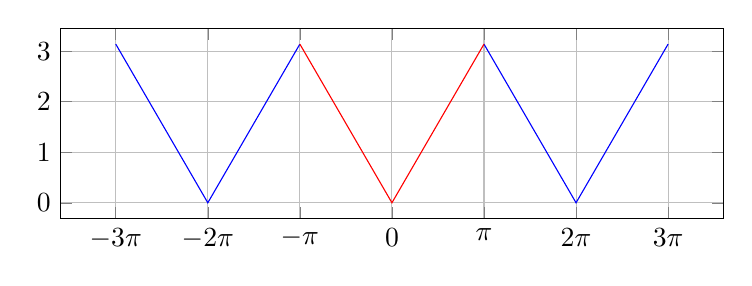
\begin{tikzpicture}
 			\pgfplotsset{width=10cm,height=4cm}
 			\begin{axis}[grid = major,xtick={-9.42,-6.28,-3.14,0,3.14,6.28,9.42},
 				xticklabels={$-3\pi$,$-2\pi$,$-\pi$,$0$,$\pi$,$2\pi$,$3\pi$}]
 				\addplot[color=blue]
 				table
 				{
 					X Y
 					-9.42 3.14
 					-6.28 0
 					-3.14 3.14
 				};
 				\addplot[color=blue]
 				table
 				{
 					X Y
 					3.14 3.14
 					6.28 0
 					9.42 3.14
 				};
 				\addplot[color=red]
 				table
 				{
 					X Y
 					-3.14 3.14
 					0 0
 					3.14 3.14
 				};
 			\end{axis}
 		\end{tikzpicture}
 	\end{minipage}
 	
 	شۇنىڭ ئۈچۈن:
 	$$
 	f(x) = |x|= \frac{\pi}{2}-\frac{4}{\pi}\sum_{n=0}^{\infty} \frac{\cos (2n-1)x}{(2n-1)^2}, \quad |x| \le \pi
 	$$
 \end{myexample}

\subsection{فۇريې ئالماشتۇرىشى}

ئالدىنقى مەزمۇنلاردا فۇريې قاتارى خاتېرلەندى، ئەمدى بىز يەنە بىر مۇھىم نۇقتا 
\textbf{فۇريې ئالماشتۇرىشى}
ھەققىدە توختىلىپ ئۆتىمىز.\\
خالىغان دەۋرىيسى $2l$ بولغان دەۋرىي فۇنكىسىيەنىڭ فۇريې قاتارى:
 
 \begin{align}
 	f(x)=\frac{a_0}{2}+\sum_{n=1}^{\infty}(a_n\cos \frac{n \pi x}{l} + b_n\sin \frac{n \pi x}{l}) \\
 	a_n = \frac{1}{l} \int_{-l}^{l}f(x) \cos \frac{n \pi x}{l} dx , n=0,1,2,... \\
 	b_n = \frac{1}{l} \int_{-l}^{l}f(x) \sin \frac{n \pi x}{l} dx , n=1,2,3,...
 \end{align}

 \begin{indicate}
 	\begin{minipage}[b]{0.85\linewidth}
 		\textbf{ئەيلېر فورمۇلىسى}
 		كەڭ ئىشلىتىلىدىغان فورمۇلا بولۇپ، كومپېلىكىس ئۆزگەرگۈچى فۇنكىسيەدىكى ئىنتايىن مۇھېم فورمۇلانىڭ بىرىدۇر. مەلۇمكى $i$ مەۋھۇم سان بىرلىكىدۇر، يەنى $i^2 = -1$ \\
 		ئەيلېر فورمۇلىسى:
 		$$e^{ix} = \cos x + i\sin x$$
 		بۇنى تەيلور يېيىلمىسى ئارقىلىقمۇ كەلتۈرۈپ چىقىرىشقا بولىدۇ. كەلتۈرۈپ چىقىرىش جەريانى قىسقارتىلدى.
 	\end{minipage}
 	\hfil
 	\begin{minipage}[b]{0.1\linewidth}
 		
\begin{tikzpicture}
 			\node[graduate,minimum size=1.5cm]{};
 		\end{tikzpicture}
 	\end{minipage}
 \end{indicate}

فورمۇلا $1.1-1.3$ لارنى ئەيلېر فورمۇلىسى بىلەن بىرىكتۈرسەك:

 \begin{align*}
f(x) &= \frac{a_0}{2}+\sum_{n=1}^{\infty}(a_n\cos \frac{n \pi x}{l} + b_n\sin \frac{n \pi x}{l}) = \frac{a_0}{2}+\sum_{n=1}^{\infty} \left[ \frac{a_n}{2} \left (e^{i\frac{n \pi x}{l}}+e^{-i\frac{n \pi x}{l}} \right)-\frac{ib_n}{2} \left (e^{i\frac{n \pi x}{l}}-e^{-i\frac{n \pi x}{l}} \right) \right] \\
&= \frac{a_0}{2}+\sum_{n=1}^{\infty} \left[ \frac{a_n-ib_n}{2}e^{i\frac{n \pi x}{l}}+\frac{a_n+ib_n}{2}e^{-i\frac{n \pi x}{l}}\right] 
= \frac{a_0}{2}+\sum_{n=1}^{\infty} \left[ \frac{a_n-ib_n}{2}e^{i\frac{n \pi x}{l}}+\frac{a_n+ib_n}{2}e^{-i\frac{n \pi x}{l}}\right] \\
&= C_0 +\sum_{n=1}^{\infty} \left[ C_ne^{i\frac{n \pi x}{l}}+C_{-n}e^{-i\frac{n \pi x}{l}}\right] = \sum_{n=-\infty}^{+\infty}C_n e^{i \frac{n \pi x}{l}},\quad C_0 = \frac{a_0}{2} , C_n=\frac{a_n-ib_n}{2},C_{-n}=\frac{a_n+ib_n}{2}
\end{align*}
دىمەك 
$$
C_n = \frac{1}{2l} \left [ \int_{-l}^{l}f(x) \cos \frac{n \pi x}{l} dx -i\int_{-l}^{l}f(x) \sin \frac{n \pi x}{l} dx \right ] = \frac{1}{2l}\int_{-l}^{l}f(x)e^{-i \frac{n \pi x}{l}} dx
$$

$C_n$
 مۇ تېپىلدى، فۇريې قاتارى مەزمۇنىدا فۇنكىسىيە دەۋرىنى $T=2l$ دېگەن. شۇڭا $\left [-\frac{T}{2},\frac{T}{2}\right ]$ ئىچىدە، فۇنكسىيە $f(x)$ نى يۇقىرىدا كەلتۈرۈپ چىقارغان فۇريې قاتارى فورمۇلىسى بويىچە مۇنداق يېزىشقىمۇ بولىدۇ:
 $$
 f_T(x) = \sum_{n= -\infty}^{+\infty}C_n e^{i \frac{2n \pi x}{T}}
 $$
 فىزىكىلىق بىلىملەرگە ئاساسەن، بۇلۇڭلۇق تىزلىك $\omega$ ۋە دەۋرىي $T$ ۋە چاستوتا $f$ ئوتتۇرسىدا مۇنداق مۇناسىۋات بار:
 \begin{align*}
\Delta \omega = \omega = \frac{2 \pi}{T}, \quad \Delta \omega = \omega_n-\omega_{n-1} \\
T = \frac{1}{f} = \frac{2\pi}{\omega}, \quad f = \frac{1}{T} = 2 \pi \omega
 \end{align*}
شۇڭا يەكۈنلەشكە بولىدۇكى:
\begin{align*}
f_T(x) &= \sum_{n=-\infty}^{+\infty}C_n e^{in \omega x} \\
C_n &= \frac{1}{T} \int_{-\frac{T}{2}}^{\frac{T}{2}} f_T(x)e^{-in \omega x}dx , n=0, \pm 1, \pm 2 , ... \\
f_T(x) &=\frac{1}{T}\sum_{n=-\infty}^{+\infty} \left (\int_{-\frac{T}{2}}^{\frac{T}{2}} f_T(x)e^{-in \omega x}dx \right)e^{in \omega x}
\end{align*}
ئۈستىدىكى ئۆز نۆۋىتىدە يەنە 
\textcolor{red}{فۇريې دەرىجىلىك قاتارى}
دەپ ئاتىلىدۇ، چۈنكى بۇنىڭ بارلىق ئەزالىرى $e$ نىڭ دەرىجىسىنىڭ ۋەزىنلىك يىغىندىلىرىدىن تۈزىلىدۇ.

\begin{colorful}[cyan]
يۇقارقى فورمۇلا ۋە ئەيلېر فورمۇلاسىنىڭ گېئومىتېريەلىك مەنىسىدىن بىلىۋىلىشقا بولىدۇكى، فۇنكىسىيە $f(x)$ نى نۇرغۇن چەمبەر بويلىما ھەركەت يايلىرىنىڭ ۋەزىنلىك يىغىندىسى دەپ قاراشقىمۇ بولىدۇ.
ئەلۋەتتە بۇ فورمۇلا سىزىقلىق ئالگېبرادىكى بىلىملەر بىلەن تامامەن بىردەك.يەنى: سىزىقلىق بوشلۇقتا بىز بىر گورۇپا ئاساس ۋېكتورلارنى تاللاپلا، بۇ بوشلۇقتىكى بارلىق ۋېكتورلارنى مۇشۇ ئاساس ۋېكتورلارنىڭ سىزىقلىق بېرىكمە شەكلىدە ئىپادىلەپ چىقالايمىز.
\end{colorful}
 
 ئادەتتە نۇرغۇن فونكىسيەلەرنىڭ دەۋرىيسى $T$ ئېنىق مەۋجۇت بولمايدۇ، ئەمما بىز بۇلارنىڭ دەۋرىيسىنى چەكسىز دەپ قارىۋالساقلا بولىدۇ.  شۇڭا ئۈستىدىكى: $\lim_{T \to + \infty}f_T(x) = f(x)$ 
 $$
 f(x) = \lim_{T \to + \infty}f_T(x) = \lim_{T \to +\infty} \frac{1}{T}\sum_{n=-\infty}^{+\infty} \left (\int_{-\frac{T}{2}}^{\frac{T}{2}} f_T(x)e^{-in \omega x}dx \right)e^{in \omega x}
 $$
 يۇقىرىدىكى لىمىت نەزىريەسى ئاساسىدا بۇ ئىپادىگە قارىتا ئاددىيلاشتۇرۇش ئېلىپ بارىمىز. دەۋرىيسى چەكسىزلىككە قاراپ ماڭدى، دىمەك بۇلۇڭلۇق تىزلىكى نۆلگە قاراپ ماڭدى دېگەنلىك.
\begin{align*}
 f(x) &= \lim_{T \to +\infty} \frac{1}{T}\sum_{n=-\infty}^{+\infty} \left (\int_{-\frac{T}{2}}^{\frac{T}{2}} f_T(x)e^{-in \omega x}dx \right)e^{in \omega x} \\
 &= \lim_{\Delta \omega \to 0}\frac{1}{2 \pi} \sum_{n=-\infty}^{+\infty} 
 \left (\int_{-\frac{T}{2}}^{\frac{T}{2}} f_T(x)e^{-i\omega_n x}dx \right) \Delta \omega
\end{align*}
چۈنكى $\Delta \omega \to 0(T \to +\infty)$ ۋەجىدىن، تۆۋەندىكىدەك ھادىسە مەۋجۇت:
\begin{align*}
\Delta &\omega \to 0(T \to +\infty) \\
\therefore \int_{-\frac{T}{2}}^{\frac{T}{2}} &\rightarrow \int_{-\infty}^{+\infty} \\
{\omega_n=n\omega} &\rightarrow {\omega=\omega_n-\omega_{n-1}} \\
\int_{-\frac{T}{2}}^{\frac{T}{2}} f_T(x)e^{-i\omega_n x}dx &\rightarrow
\int_{-\infty}^{+\infty} f(x)e^{-i\omega x}dx = F(\omega)
\end{align*}
شۇڭلاشقا:
\begin{align*}
f(x) &= \frac{1}{2 \pi} \int_{-\infty}^{+\infty}F(\omega)e^{i \omega x}d\omega \\
F(\omega) &= \int_{-\infty}^{+\infty} f(x)e^{-i\omega x}dx \\
\therefore f(x) &= \frac{1}{2 \pi} \int_{-\infty}^{+\infty}\left [ \int_{-\infty}^{+\infty} f(x)e^{-i\omega x}dx \right]
e^{i \omega x}d\omega
\end{align*}

مانا ئەڭ ئاخرىدىكى فورمۇلانى بىز فۇريې ئىنتىگىرال فورمۇلاسى دەيمىز.

ئەگەر فۇنكىسىيە $f(x)$ ئىنتېرۋال $[-\infty,+\infty]$ مۇتلەق ئىنتېگىراللىغىلى بولسا، يۇقىرىدىكى $F(\omega)$ نى بىز فۇنكىسىيە $f(x)$ نىڭ 
\textcolor{red}{فۇريې ئالماشتۇرىشى}
دەيمىز. ھەم تۆۋەندىكىدەك خاتېرلەيمىز:

\begin{align*}
F(\omega) &= F[f(x)] \\
F[f(x)] &= \int_{-\infty}^{+\infty} f(x)e^{-i\omega x}dx
\end{align*}

مانا بۇ فۇريې ئالماشتۇرىشى.\\
ئالماشتۇرۇشتى كىيىنكى فۇنكىسىيەنى ئەسلىي فۇنكىسىيە بىلەن بىرلەشتۈرۈپ فۇريې تەتۈر ئالماشتۇرىشى دەپ ئاتايمىز.  ھەم تۆۋەندىكىدەك خاتىرلەيمىز:

\begin{align*}
f(x) &= F^{-1}[F(\omega)] \\
f(x) &= F^{-1}[F(\omega)] \\
F^{-1}[F(\omega)] &= \frac{1}{2 \pi} \int_{-\infty}^{+\infty}F(\omega)e^{i \omega x}d\omega
\end{align*}

فۇريې قاتارى ۋە فۇريې ئالماشتۇرىشىنىڭ مۇناسىۋىتى: فۇريې قاتارى ئارقىلىق ھەرقانداق دەۋرىي فۇنكىسىيەنى ئىپادىلىگىلى بولىدۇ، ئەگەر فۇنكسىيە دەۋرىي فۇنكىسىيە ئەمەس بولسا، ئۇنداقتا ئۇنىڭ دەۋرى چەكسىز ئېنتېرۋال ئىچىدە بولىدۇ. دەۋرى چەكسىزلىككە ماڭسا بۇلۇڭلۇق تىزلىق 0 گە قاراپ ماڭىدۇ شۇنداقلا ئاساس چاستوتىسى 0 گە قاراپ ماڭىدۇ، بۇ ۋاقىتتا چاستوتىسى داۋاملىق دىسكرېت ھالەتتە بولماي ئۈزلۈكسىز ھالەتتە بولىدۇ دە فۇريې ئالماشتۇرىشى ئارقىلىق داۋاملىق تەھلىل قىلغىلى بولىدۇ.

\begin{colorful}[red]
فۇريېنىڭ قىياسى: ھەرقانداق دەۋرىي فۇنكىسىيەنى تروگونومېتىرىيىلىك فۇنكسىيەلەرنىڭ يىغىندىسى يەنى فۇريې قاتارى ئارقىلىق ئىپادىلىگىلى بولىدۇ.
\end{colorful}

\subsection{دىسكرېت فۇريې ئالماشتۇرىشى}
يۇقىرىدىكى كۆپلىگەن باسقۇچلاردىن كىيىن، بىز ئېرىشكەن فۇريې دەرىجىلىك قاتارى ۋە فۇريې ئالماشتۇرىشى تۆۋەندىكىدەك:
\begin{align*}
f(x) &= \sum_{n=-\infty}^{+\infty}C_n e^{in \omega x} \\
F(\omega) &= \int_{-\infty}^{+\infty} f(x)e^{-i\omega x}dx \\
f(x) &= \frac{1}{2 \pi} \int_{-\infty}^{+\infty}F(\omega)e^{i \omega x}d\omega\\
\end{align*}
ئەمما ھېساپلاش ماشىنىسى پەقەت چەكلىك ئېقىمدىكى ئۇچۇرلارنى بىرتەرەپ قىلالايدۇ، يەنە كىلىپ ئۈزلۈكسىز دائىرىدىكى ئۇچۇرلارنى ئەسلا بىر تەرەپ قىلايلمايدۇ. شۇڭا فۇريې ئالماشتۇرشىنى چوقۇم چەكلىك بولغان دىسكرېت ھالەتكە ئايلاندۇرۇش كېرەك.
$$e^{ki \frac{2 \pi}{D} n}$$
دىسكرېت ئالماشتۇرىشى بىرتەرەپ قىلىدىغىنى دىسكرېت دەۋرىي سىگنال. ئالايلۇق بىز سىگنال تەرتىپلىرى $\{ x[1],x[2],x[3],... \}$ دەۋرىيسىنى $D$ دەپ قارايلى، ئۇنداقتا خالىغان پۈتۈن سان $r$ غا نىسبەتەن، بىر پۈتۈن دەۋرىي ئىچىدىكى سىگناللار تەڭداش، يەنى $x[n] = x[n+rD]$ .

ئۈزلۈكسىز سىگنال مەيدانىدا فۇريې بوشلۇقىدىكى ئاساس $e^{ki \omega t}$ بولۇپ، $k$ پۈتۈن ساننى ئىپادىلەپ ئوخشىمىغان ئاساسنى بەلگىلەپ قويىدۇ، $t$ بولسا ۋاقىت ئۈزلۈكسىز مىقدارى.

ھازىر بىزنىڭ قىلىدىغىنىمىز دىسكرېت ھەم دەۋرىي سىگنال، دەۋرىيسى $D$ , شۇڭا ۋاقىت مىقدار دىسكرېت سىگنال تەرتىپى $n$ گە ئايلىنىدۇ. شۇنىڭ بىلەن بۇ دىسكرېت بوشلۇقتىكى ئاساس $e^{ki \frac{2 \pi}{D} n}$ غا ئۆزگىرىدۇ. شۇڭا فۇريې ئالماشتۇرىشى تۆۋەندىكىدەك ئۆزگىرىدۇ:

ئۈزلۈكسىز: ئەسلىدىكى سىگنال $f(x)$ 
\begin{align*}
C_k = \frac{1}{T} \int_{-\frac{T}{2}}^{\frac{T}{2}} f(t)e^{-ki \omega t}dt , k=0, \pm 1, \pm 2 , \pm 3, ... \\
f(t) = \sum_{k=-\infty}^{+\infty}C_k e^{ki \omega t}
\end{align*}
دىسكرېت: ئەسلىي سىگنال $x[n]$ 
\begin{align*}
X_k = \sum_{n=0}^{D-1}x[n] e^{-ki \frac{2 \pi}{D} n}
\\
x[n] = \frac{1}{D}\sum_{k=0}^{D-1}X_k e^{ki \frac{2 \pi}{D} n}
\end{align*}
بۇ يەكۈنگە ئەيلېر فورمۇلاسىنى بىرلەشتۈرۈپ 
$w = e^{2 \pi i/D} = \cos \frac{2 \pi}{D} -i \sin \frac{2 \pi}{D}$ 
$x=FX$
 شەكلىدىكى سىزىقلىق تەڭلىمىلەر سېستىمىسىغا ئېرشەلەيمىز، يەنى:
\begin{align*}
 \begin{bmatrix}
	x[0] \\
	x[1] \\
	x[2] \\
	\vdots \\
	x[X-1]
\end{bmatrix} 
=
\begin{bmatrix}
	1& 1& 1& \cdots & 1 \\
	1& w& w^2& \cdots & w^{N-1} \\
	1& w^2& w^4& \cdots & w^{2(N-1)} \\
	\vdots & \vdots & \vdots & \ddots & \vdots &\\
	1& w^{N-1}& w^{2(N-1)}& \cdots & w^{(N-1)^2} \\
\end{bmatrix}
\begin{bmatrix}
	X_0 \\
	X_1 \\
	X_2 \\
	\vdots \\
	X_{N-1}
\end{bmatrix}
\end{align*}

ئەلۋەتتە، ئۈستىدىكى ماترىسسا 
\textcolor{red}{ۋاندېرموند ماترىسسا}
ۋە ياكى 
\textcolor{red}{ فۇريې ماترىسسا}
دەپمۇ ئاتىلىدۇ. مۇشۇ ماترىسسانىڭ خۇسۇسىيتى دەل دىسكرېت فۇريې ئالماشتۇرشىنىڭ ئالاقە رەقەملىك ئۇچۇرنى بىرتەرەپ قىلغىلى بولىدىغان بولمايدىغانلىقىنى بەلگىلەپ قويىدۇ. ناۋادا بۇ ماترىسسانىڭ شەكلى ئىنتايىن مۇرەككەپ ھەتتا ئەكىس ماترىسساسى مەۋجۇت ئەمەس، ئۇنداقتا بۇنىڭ چوڭ كېرىكى قالمايدۇ. ئەلۋەتتە، بۇ ماترىسسانىڭ ئۆزى ياكى ئەكىس ماترىسساسىنىڭ ھېساپلاشلىرىنى تىز ئېلىپ بېرىش ئۈچۈن مەيدانغا 
  \textbf{تىز فۇريې ئالماشتۇرشى}
   مەيدانغا كىلىدۇ. قسىقىسى دىسكرېت فۇريې ئوڭ-تەتۈر ئالماشتۇرۇشلىرىنى ھېساپلاشتا ئىشلىتىلىدۇ.

\begin{myexample}
	كۇۋادىرات دولقۇننى دەۋرىيسى $2\pi$ بولغان سىگنالنىڭ ئىنتېرۋال $[-\pi,\pi]$ ئىچىدىكى فۇنكىسىيە ئىپادىسى تۆۋەندىكىچە:
	$$g(x) = 
	\begin{cases}
		1 ,\quad 0 < x < \pi \\
		-1 , \quad -\pi < x < 0
	\end{cases}
	$$
	\rule{\linewidth}{0.05em}\\
	فۇريې قاتارى فورمۇلىسىگە ئاساسەن، ھېساپلاپ چىقىشقا بولىدۇكى:
\begin{align*}
a_n &= \frac{1}{\pi} \int_{-\pi}^{\pi}g(x) \cos \frac{n \pi x}{\pi} dx 
= \frac{2}{\pi} \int_{0}^{\pi}\cos nxdx = 0, \quad n=0,1,2,...\\
b_n &= \frac{1}{\pi} \int_{-\pi}^{\pi}g(x) \sin \frac{n \pi x}{\pi} dx
= \frac{2}{\pi} \int_{0}^{\pi}\sin nxdx = \frac{2}{n\pi}(1-\cos n\pi), \quad n=0,1,2,...
\end{align*}
شۇڭا بۇ سىگنالنىڭ فۇريې قاتارى ئارقىلىق ئىپادىلىنىشى مۇنداق:
$$
F(x)=\sum_{n=1}^{\infty}(b_n\sin \frac{n \pi x}{l}) = \frac{2}{\pi} \sum_{n=1}^{\infty}(\frac{1-\cos n\pi}{n} \sin nx)
$$
\end{myexample}









\newpage
\mychapter{دىففېرېنسىئال تەڭلىمە}
\par\bigskip
\begin{tcolorbox}
تەڭلىمە ئۇقۇمى باشلانغۇچ ماتېماتىكىسىدا ئەڭ بۇرۇن ئۇچرايتتى. ئىلگىرىكى مەزمۇنلاردا فۇنكسىيە، ھاسىلە ئۇقۇمى، دىففېرېنسىئال ۋە ئىنتېگرال ئۇقۇملىرىنى ئىگەللىگەندىن كىيىن مۇشۇلارنىڭمۇ تەڭلىمىگە ئائىت قوللىنىشلىرىنى بىلىش ئۈچۈن، شۇنداقلا تۇرمۇشتىكى ئەمەلىي مەسىلىلەرنىڭ ئېھتىياجى ئۈچۈن تۆۋەندە يېڭى بىر بىلىم نۇقتىسى بىلەن تونۇشۇپ چىقىمىز. بۇ باپتا بىر قەدەر قىيىن بولغان نۇقتا
\textbf{دىففېرېنسىئال تەڭلىمە}
ھەققىدە دەسلەپكى بىلىملەرنى ئۆگىنىپ چىقايلى.

\end{tcolorbox}
\section{دىففېرېنسىئال تەڭلىمە}
\subsection{ئاساسىي ئۇقۇم}

\begin{MyDefinition}{دىففېرېنسىئال تەڭلىمە}{}
	نامەلۇم فۇنكىسىيە ۋە نامەلۇم فۇنكىسىيە ھاسىلىسىنىڭ ئۆزگەرگۈچى مىقدار ئارىسىدىكى مۇناسىۋىتىنى ئىپادىلەيدىغان تەڭلىمە. يەنى فۇنكىسىيە ھاسىلىسىنى ئۆز ئىچىگە ئالغان تەڭلىمە دىففېرېنسىئال تەڭلىمە دەپ ئاتىلىدۇ. بۇنى 
	$$F(x,y,y^{'},...,y^{(n)})=0$$
	ئارقىلىق خاتېرلەشكە بولىدۇ.
\end{MyDefinition}
دىففېرېنسىئال تەڭلىمىدىكى نامەلۇم فۇنكىسىيە ھاسىلىسىنىڭ دەرىجىسى، دىففېرېنسىئال تەڭلىمىنىڭ \textbf{دەرىجىسى} دەپ ئاتىلىدۇ.

\subsubsection{دىففېرېنسىئال تەڭلىمىنىڭ يېشىمى}
ئەگەر فۇنكىسىيە $y=\phi(x)$ نىڭ $n$ دەرىجىلىك ئۈزلۈكسىز ھاسىلىسى $\phi^n(x)$ ، بېرىلگەن ئىنتېرۋال $I$ دا مەۋجۇت ھەم تەڭلىمە
$$F(x,\phi(x),\phi^{'}(x),...,\phi^{(n)}(x))=0$$
نى قانائەتلەندۈرسە، ئۇنداقتا فۇنكىسىيە $y=\phi(x)$ تەڭلىمە
$$F(x,\phi(x),\phi^{'}(x),...,\phi^{(n)}(x))=0$$
نىڭ ئىنتېرۋال $I$ دىكى \textbf{يېشىمى} دەپ ئاتىلىدۇ. 
\subsubsection{ئومۇمىي يېشىمى}
ئەگەر دىففېرېنسىئال تەڭلىمە يېشىمى خالىغان تۇراقلىق ساننى ئۆز ئىچىگە ئالغان ھەمدە خالىغان تۇراقلىق ساننىڭ سانى تەڭلىمە دەرىجىسى بىلەن تەڭ بولغاندا، بۇ يېشىمىنى تەڭلىمىنىڭ \textbf{ئومۇمىي يېشىمى} دەپ ئاتايمىز.
\subsubsection{ئالاھېدە يېشىمى}
دىففېرېنسىئال تەڭلىمە ئومۇمىي يېشىمىدىكى خالىغان تۇراقلىق ساننى مۇقىم بېكىتكەندىن كىيىن ئېرىشكەن يېشىمنى، \textbf{ئالاھىدە يېشىمى} دەپ ئاتايمىز.

\subsection{ئاساسىي تەڭلىمىلەر}
\begin{itemize}
\item \textbf{دەسلەپكى قىممەت شەرتى}\\
ئەگەر $x=x_0$ بولغاندىكى فۇنكىسىيە ۋە ئۇنىڭ ھاسىلىسىنىڭ قىممىتى $y_0,y_{0}^{'}$ بېرىلگەن بولسا، بۇنداق شەرتلەرنى بىز تەڭلىمىنىڭ دەسلەپكى قىممەت شەرتى دەپ ئاتايمىز.
\item \textbf{بىرىنچى دەرىجىلىك دەسلەپكى قىممەت مەسىلىسى}\\
تەڭلىمە $y^{'}=f(x,y)$ نىڭ دەسلەپكى شەرت $y|_{x=x_0}=y_0$ ئاستىدىكى ئالاھېدە يېشىمىنى تېپىش مەسىلىسىنى كۆرسىتىدۇ. يەنى:
$$
\left\{\begin{array}{l}
y^{'} = f(x,y) \\
y|_{x=x_0}=y_0
\end{array}\right.
$$

\item \textbf{ئىككىنچى دەرىجىلىك دەسلەپكى قىممەت مەسىلىسى}\\
تەڭلىمە $y^{''}=f(x,y,y^{'})$ نىڭ دەسلەپكى شەرت $y|_{x=x_0}=y_0, y^{'}|_{x=x_0}=y_{0}^{'}$ ئاستىدىكى ئالاھېدە يېشىمىنى تېپىش مەسىلىسىنى كۆرسىتىدۇ. يەنى:
$$
\left\{\begin{array}{l}
y^{''}=f(x,y,y^{'}) \\
y|_{x=x_0}=y_0, y^{'}|_{x=x_0}=y_{0}^{'}
\end{array}\right.
$$
\item \textbf{پارچىلىغىلى بولىدىغان تەڭلىمە}\\
شەكلى تۆۋەندىكىدەك بولغان تەڭلىمىنى پارچىلىغىلى بولىدىغان تەڭلىمە دەپ ئاتايمىز:
$$
y^{'}=f(x)g(y)
$$
\end{itemize}

سالام دۇنيا.
%%%%%%%%%%
\begin{myexample}
	تەڭلىمە
	$\dfrac{dy}{dx}=2xy$
	نى يېشىڭ.
	\\\rule{\linewidth}{0.05em}\\
	كۆرۈۋېلىشقا بولىدۇكى، بۇ بىر پارچىلىغىلى بولىدىغان تەڭلىمە.\\
$$\displaystyle{\int\dfrac{dy}{y}}=\int2x\,dx, \ln\vert y\vert=x^2+C, \vert y\vert=e^{x^2+C}$$
$$\therefore y=\pm e^{x^2}e^C=\pm C_1e^{x^2}=C_2e^{x^2}$$
\end{myexample}



\section{ئادەتتىكى دېففېرېنسىئال تەڭلىمە}
\subsection{سىزىقلىق دىففېرېنسىئال تەڭلىمە}
\subsection{بېرنوئىل تەڭلىمىسى}
\subsection{تۆۋەنلەتكىلى دېففېرېنسىئال تەڭلىمە}

\section{يۇقرى دەرىجىلىك سىزىقلىق دىففېرېنسىئال تەڭلىمە}
\subsection{يۇقرى دەرىجىلىك تەڭلىمە}
\subsection{ئەيلېر تەڭلىمىسى}



%%%%%%%%%%%%%%%%%%%%%%%%%%%%%%%%%%%%%%%
%\setcounter{part}{1}
\part{ئالگېبرا}
\newpage
\mychapter{دېتېرمىنانت}

\section{ئۇقۇم}
\subsection{ئالاھېدە دېتېرمىنانىت}

\section{ھېساپلاش}
\subsection{تولدۇرغۇچى مىنور}
\subsection{ئالگېبرالىق تولدۇرغۇچى مىنور}
\subsection{دېتېرمىنانىتنى يېيىش قائىدىسى}

\newpage
\mychapter{ۋېكتور}
بۇ بۆلەك تولۇقلىنىلىۋاتىدۇ.

\section{ۋېكتور ۋە ۋېكتور ئۇقۇمى}
\subsection{ۋېكتور}
\subsection{ھېساپلاشلار}
\subsection{سىزىقلىق باغلىنىشلىق ۋېكتور}

\section{ۋېكتور خۇسۇسىيەتلىرى}
\subsection{ۋېكتور سىزىقلىق مۇناسىۋەتسىزلىك}
\subsection{ۋېكتور رانكى}
\subsection{ۋېكتور تەڭداشلىقى}
\subsection{ۋېكتور بوشلۇقى}

\newpage
\mychapter{ماترىسسا}

\section{ئاساسىي ئۇقۇم}
\subsection{ماترىىسا ئارىسىدا ھېساپلاش}
\subsection{ماترىسسا خۇسۇسىيەتلىرى}

\section{ماترىسسا خاسلىقلىرى}
\subsection{ماترىسسا ۋە دېتېرمىنانىت}
\subsection{ماترىسسا رانكى}
\subsection{خاراكتېرلىگۈچى قىممەت ۋە ۋېكتور}


\section{ئالاھېدە ماترىسسالار}
\subsection{ئېلمىنتار ماترىسسا}
\subsection{تەتۈر ماترىسسا}
\subsection{تەڭداش ماترىسسا}
\subsection{سىممىتېرىك ماترىسسا}
\subsection{ئوخشاش ماترىسسا}
\subsection{ئورتوگىنال ماترىسسا}

%%%%%%%%%%%%%%%%%%%%%%%%%%%%%%%%%%%%%%%

%%%%%%%%%%%%%%%%%%%%%%%%%%%
\part{ئېھتىماللىق نەزىرىيىسى}

%\input{AdvancedMath/}
%\input{Probability/}
%\input{LinearAlgebra/}


\newpage
\section*{مەشىقلەرنىڭ پايدىلىنىش جاۋاب كودى}
%\tcbinputrecords  %Write recorded answer

\newpage
%\input{chapter/appdix.tex}

%\newpage
%\listoftables

%\newpage
%\listoffigures

%\section{پايدىلانمىلار}


\begin{thebibliography}{9}
\begin{english}
	\bibitem{latexcompanion} 
	\textenglish{
	Michel Goossens, Frank Mittelbach, and Alexander Samarin. \\
	\textit{The \LaTeX\ Companion}. 
	Addison-Wesley Reading Mass, 2004.
	}
	\bibitem{einstein} 
	\textenglish{
	Hubert Partl, Irene Hyna, and Elisabeth Schlegl. 
	\url{https://www.ctan.org/tex-archive/info/lshort/english}
	}
	\bibitem{einstein} 
	\textenglish{
	Jean Pierre Casteleyn. Visual TikZ (version 0.62). IUT Génie Thermique et
Énergie, 2016
	}
	\bibitem{einstein} 
	\textenglish{
	Leslie Lamport. \LaTeX: A Document Preparation System, 2nd edition.
Addison-Wesley Reading Mass, 1994.
	}
	\bibitem{einstein} 
	\textenglish{
	Till Tantau. TikZ PGF Manual, 2010. \url{http://www.ctan.org/
tex-archive/graphics/pgf/.}
	}
	\bibitem{einstein} 
	\textenglish{
	URL \url{https://texample.net/}
	}
	\bibitem{einstein} 
	\textenglish{
	URL \url{https://www.latex-project.org}
	}
	\bibitem{einstein} 
	\textenglish{
	URL \url{https://python.org/}
	}
	\bibitem{einstein} 
	\textenglish{
	URL \url{https://www.latexstudio.net/}
	}
\end{english}
\end{thebibliography}

\end{document}